\chapter[Real-Time Reorienting During Episodic Retrieval Rescues Memories]{Real-Time Reorienting During Episodic Retrieval Rescues Memories from Suboptimal Arousal-Attentional States}\label{ch:prism}

Moment-to-moment fluctuations in preparatory attention and arousal explain, in part, why certain moments are more conducive to successful memory than others \parencite{robison2022pupillary,miller2020variation,miller2019individual,cohen2015peri,madore2022readiness,madore2020memory,cohen2020prestimulus,evans2019preretrieval,curran2004effects,craik1996effects,baddeley1984attention,anderson1995status,soravia2016prestimulus,schwartz2025attending}. Evidence from neuroimaging, electrophysiology, and pupillometry indicates that such fluctuations reflect systematic shifts in the brain's arousal and attentional states — henceforth, `A-A states' — including states modulated by the locus coeruleus-norepinephrine (LC-NE) system \parencite{costa2016more,joshi2016relationships,sara2009locus,munn2021ascending,murphy2011pupillometry,murphy2014pupil,hong2014your,groot2021probing,huang2024locus}. Correlations between read-outs of A-A states, cognitive control, and memory motivate readiness-to-learn and readiness-to-remember frameworks \parencite{madore2022readiness,madore2020memory,schwartz2025attending,morcom2002getting}, which build on a rich literature linking preparatory states to cognitive performance \parencite{awh2012top,corbetta2002control,corbetta2008reorienting,debettencourt2018forgetting,fortenbaugh2015sustained,uncapher2009selecting,waskom2014frontoparietal,yoo2012when,aly2017how,strunk2019prestimulus,badre2018frontal,esterman2013zone,compton2019wandering,turnbull2019ebb,joshi2020pupil}. Notably, the apparent effects of A-A states at the time of retrieval highlight fundamental challenges for education, clinical populations with attention dysregulation, and everyday cognitive performance: well-encoded memories are not sufficient for performance if attention and arousal fluctuations in the moment just prior to an attempt to remember decrease the probability of successful memory retrieval.

The adaptive gain theory of LC function suggests that the relationship between tonic arousal/attention and cognitive performance follows an inverted-U shaped curve \parencite{astonjones2005integrative,astonjones2005adaptive,yerkes1908relation}. Pupil size, a non-invasive and continuous index of LC-NE activity, tracks fluctuations in arousal and attention with relatively high temporal resolution \parencite{beatty1982taskevoked,unsworth2018tracking,unsworth2017importance,eckstein2017beyond,konishi2017when}. Both tails of the pupil distribution have been linked with distinct modes of attentional failure. Relatively small pre-stimulus pupil size may reflect a hypoactive LC mode characteristic of internally-oriented inattention and mind wandering, whereas comparatively larger pre-stimulus pupil size might index a hyperactive LC mode associated with external distraction and exploratory disengagement \parencite{unsworth2018tracking,unsworth2016pupillary}. Greater variability in pre-stimulus pupil size has likewise been related to poorer performance both within and across participants \parencite{unsworth2018tracking,unsworth2017importance,robison2019pupillometry}, consistent with the view that frequent departures away from an intermediate arousal optimum can be detrimental to sustained cognitive engagement and performance. During cognitively demanding task sessions, tonic arousal is typically elevated, and the range of pre-stimulus pupil fluctuations observed within a session likely reflects variation around the lower and upper portions of the arousal/attention continuum rather than sampling from its true physiological extremes where relative deviations in pre-stimulus pupil size are associated with meaningful variation in memory performance \parencite{madore2022readiness,madore2020memory,sara2009locus,pitem2025predicting,kafkas2024eyes,kucewicz2018pupil,kuipers2022variations,mather2011arousal,clewett2018locus,sara2015locus}. In humans, a wealth of evidence documents how A-A processes and states during the act of retrieval itself can impact memory outcomes \parencite{cabeza2008parietal,mecklinger2010control,hutchinson2015increased,eichenbaum2017memory,sestieri2017contribution,rugg2018ventral,ciaramelli2020space,anderson2021active}, with complementary evidence from animal models and pharmacological studies suggesting that the LC-NE system plays an important role during memory retrieval such as norepinephrine-modulated hippocampal pattern completion \parencite{bliss1983reduction,hansen2015hippocampal}.

More recently, the field has focused on measuring and understanding the preparatory mechanisms that immediately precede acts of retrieval and correlate with memory outcomes (i.e., readiness-to-remember). These include read-outs of arousal, attention, and/or goal state processes just prior to and during expression of episodic memories \parencite{robison2022pupillary,miller2020variation,miller2019individual,cohen2015peri,madore2022readiness,madore2020memory,schwartz2025attending,xue2025strong}. A primary aim of the present study is to complement traditional correlational approaches to characterizing the relationship between preparatory A-A states and retrieval performance, using a closed-loop approach to garner causal evidence for the role of A-A states in episodic retrieval. To do so, we developed the PRISM (Pupil-based Real-time Intervention System for Memory) paradigm, a closed-loop pupillometry system that enables real-time monitoring of and intervention on A-A states at retrieval. PRISM continuously monitors tonic pupil diameter — an index of tonic LC-NE A-A state — in the moments just prior to each memory retrieval trial, detects A-A-defined suboptimal states (SOS) in real time via fluctuations in tonic pupil within a block, and, on a subset of trials, triggers delivery of a visual reorienting cue designed to phasically perturb the A-A state before the retrieval probe appears (Fig.~\ref{fig:closed-loop-fig1}a). This design creates a within-subject, within-session comparison between SOS trials that did not receive intervention and optimal state (OS) trials, between SOS trials that did vs. did not receive intervention, and — by leveraging the sign of the pupil deviation — between suboptimal states that the inverted-U framework predicts should differ in their amenability to recovery, enabling causal inference about the role of pre-retrieval A-A state in memory retrieval performance. 

We hypothesized that real-time triggering on SOS trials prior to retrieval will yield better memory performance than untriggered SOS trials, providing causal evidence that phasic perturbation during A-A-defined suboptimal states at retrieval rescues memory access as consistent with the readiness-to-remember framework \parencite{madore2022readiness,madore2020memory,schwartz2025attending}. Moreover, because pupil-defined SOS trials can reflect either abnormally low arousal (pupil constriction) or abnormally high arousal (pupil dilation), and because the intervention is a brief alerting stimulus that we predicted would boost phasic arousal, we further hypothesized that the theoretical inverted-U relationship between arousal and performance \parencite{yerkes1908relation} would result in an asymmetric influence of the intervention. Specifically, we hypothesized that the intervention would be effective for low-arousal SOS trials, which can be nudged toward the peak of A-A optimality, whereas the intervention may have no effect or be counterproductive for high-arousal SOS trials, which already sit on the descending limb and thus additional arousal may be ineffective or disruptive.

To test these hypotheses, we leveraged real-time readouts of trial-by-trial pupil size to detect suboptimal and optimal A-A states and to trigger, on a subset of SOS trials, a reorienting probe just prior to the retrieval attempt. After completing a goal-directed memory encoding task (Fig.~\ref{fig:closed-loop-fig1}a), participants (\textit{n}=67) encountered studied and novel items and engaged in episodic retrieval. Specifically, on each retrieval trial, participants indicated whether they remembered the test probe as having been encountered in one of the two orienting tasks during encoding, they recognize the probe as having been studied but cannot remember the orienting task, or they perceive the probe as novel. Memory for studied items was assayed at the trial-level (hits/misses) and overall condition-level performance was computed using item memory \textit{d'} and associative memory \textit{d'} (Fig.~\ref{fig:closed-loop-fig1}c). 

Using PRISM to detect and intervene on suboptimal preparatory A-A states, at the beginning of each retrieval block, we built participant-specific distributions of baseline-pupil during tonic fixation periods, which we used to establish the trigger threshold for that block. Subsequently, we computed pupil size during the 2.4-3.4s preceding each retrieval trial to detect, in real time, whether moment-to-moment pupillary dilation/constriction exceeded or fell within the empirical threshold, thus marking a trial as a SOS or OS event (Fig.~\ref{fig:closed-loop-fig1}b). On 50\% of SOS trials, PRISM triggered deployment of a salient, real-time arousal/attention-reorienting cue just prior to retrieval probe delivery. This design yielded three within-subjects conditions at retrieval: \textit{OS trials} (optimal arousal/attention maintained throughout the real-time monitoring window; no intervention needed), \textit{SOS trials with trigger} (suboptimal A-A state detected and arousal/attention reorienting cue delivered), and \textit{SOS trials without trigger} (suboptimal A-A state detected but no reorienting cue delivered).  Trigger and no-trigger SOS conditions were balanced by design via adaptive randomization. On each lapse trial, if the cumulative trigger/no-trigger distribution was at parity (50/50), assignment was determined by a random coin flip. When the cumulative proportion of either condition exceeded 50\%, the next lapse trial was deterministically assigned to the underrepresented condition, after which the system reverted to random assignment upon reaching equilibrium. This ensured that the cumulative distribution never deviated by more than one trial from parity while preserving local stochasticity (i.e., the algorithm could produce short runs of the same assignment at equilibrium, preventing strict alternation). Non-lapse trials did not interact with the trigger assignment system and thus did not affect the trigger/no-trigger sequence.

The binary classification of trials as SOS or OS belies a potentially more nuanced reality; the inverted-U framework implies that A-A states vary continuously and that suboptimal states differ in severity. That is, some represent moderate deviations from a peak A-A state and may reflect SOS states that remain within a recoverable range, while others represent extreme departures where intervention may be insufficient to restore performance. PRISM's real-time detection algorithm, which applies a fixed threshold to tonic pupil diameter in real-time, treats all threshold crossings equivalently. Theoretically, a trial that minimally crosses the lapse boundary may occupy a fundamentally different position on the A-A continuum than one representing a deep departure (see Fig.~\ref{fig:closed-loop-fig4}). Moreover, because tonic pupil size exhibits slow non-stationary drift over the course of each run, it is likely some threshold crossings are driven primarily by drift rather than putative A-A state changes.

We exploited this property to operationalize the severity continuum. By applying a post hoc spline drift correction to the pupil timeseries, we reclassified each trial's A-A state against drift-corrected thresholds (see Section~\ref{sec:methods}). Furthermore, we then distinguished trials whose real-time SOS classification was driven by drift (i.e., representing putative moderately suboptimal states closer to the peak of the inverted-U) from those whose classification survived the correction (i.e., those representing putative deep suboptimal states further from the peak). This reclassification, when crossed with trigger delivery, yielded a six-cell gradient of inferred A-A state quality that enabled post hoc testing of whether the trigger's functional impact scales with position on the continuum, conferring greater benefit to moderately suboptimal states where the fixed-magnitude perturbation may be sufficient to nudge the state toward peak optimality, and lesser benefit to deeply suboptimal states where the same perturbation may be insufficient to bridge the larger distance. Moreover, because the reclassification preserves the sign of the pupil deviation (constriction vs. dilation), it also enabled a direct test of the directional asymmetry hypothesis, which predicts that the A-A-boosting trigger would selectively rescue low-A-A (constriction) SOS trials, which sit on the ascending limb of the inverted-U and can be nudged toward the peak, but not high-A-A (dilation) SOS trials, which sit on the descending limb where additional arousal/attention may be ineffective or counterproductive.

\begin{figure}[ht!]
	\centering
	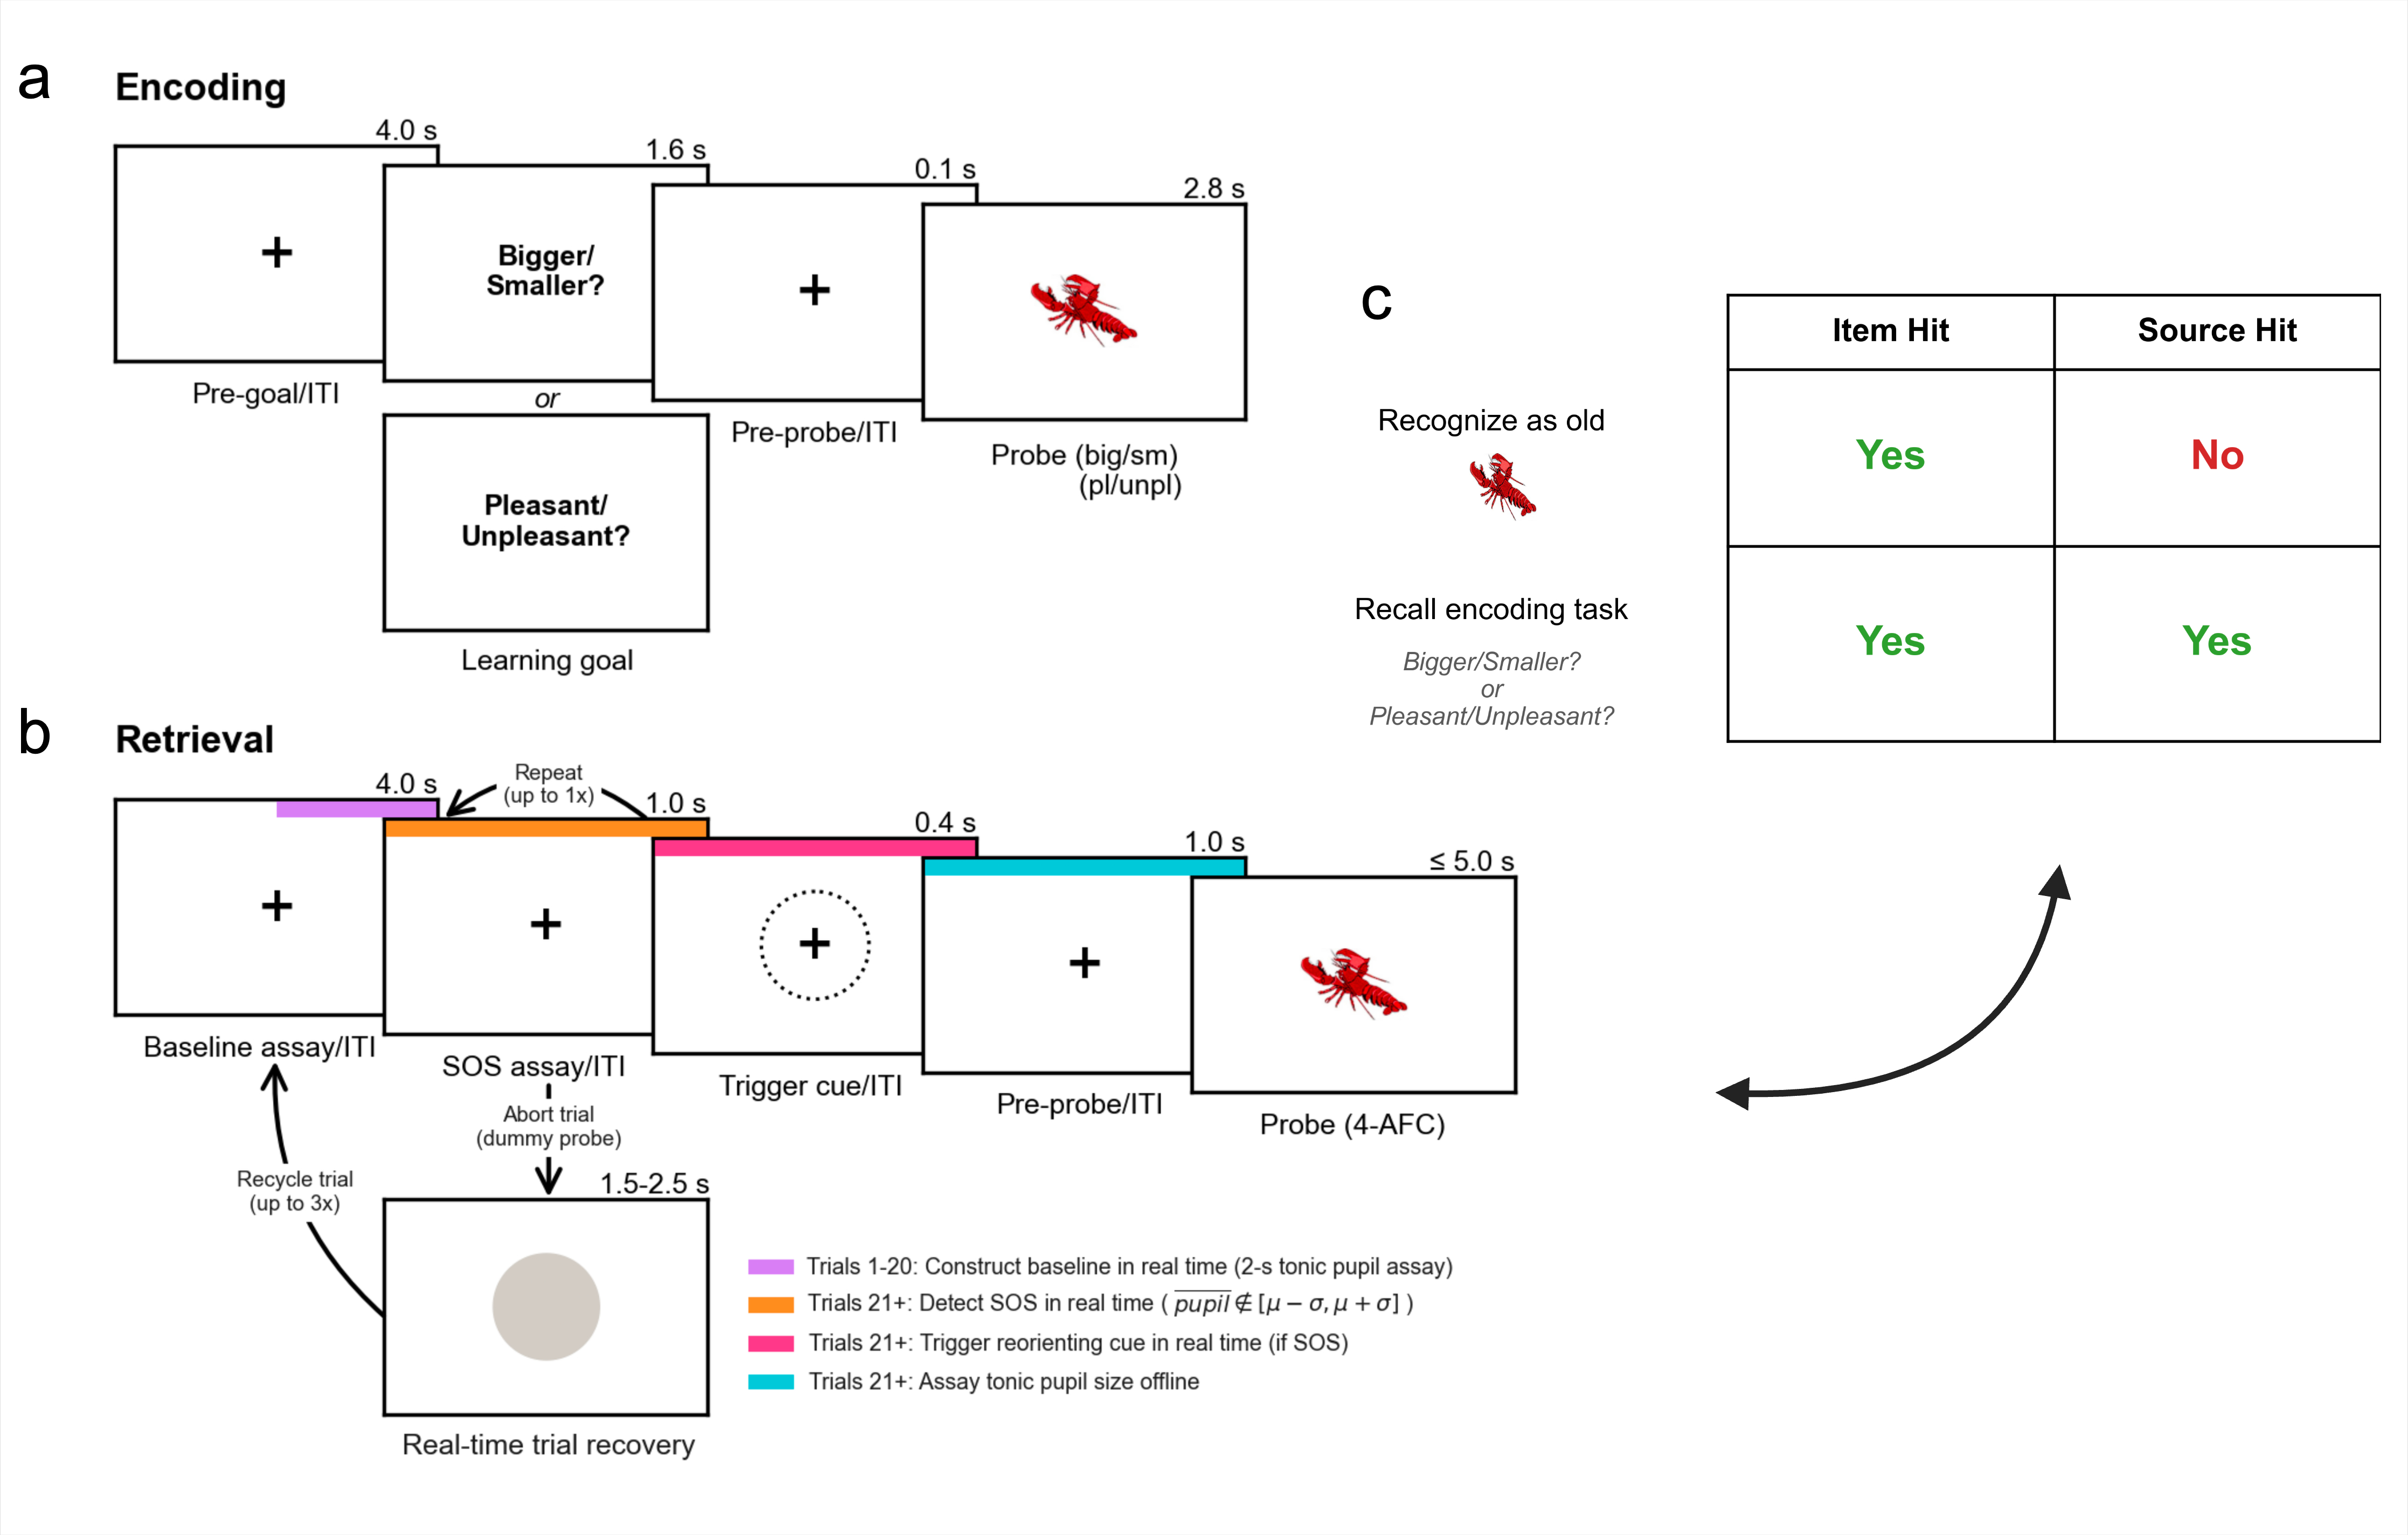
\includegraphics[width=1\linewidth]{figures/closed-loop-fig1.jpg}
	\caption[PRISM’s real-time experimental design]{PRISM’s real-time experimental design. (a) Participants viewed 168 objects once across 3 intentional encoding runs of 56 trials each. In each encoding run, 28 objects were classified on a conceptual goal dimension (pleasant or unpleasant) and 28 on a perceptual dimension (bigger or smaller), yielding 84 conceptual object trials and 84 perceptual object trials across runs. Each object appeared either bigger (450×450 px) or smaller (150×150 px) in size on the screen, independent of goal cue, counterbalanced across participants through random assignment. (b) After each encoding run, participants performed a retrieval run for the just-encoded objects, wherein they viewed 84 objects –– 56 studied and 28 novel foils. On each trial, participants made a four-alternative forced-choice (4-AFC) memory judgment on a medium-sized object (300×300 px), indicating whether they: (1) remember performing the size decision (i.e., bigger or smaller before) with the object, (2) remember performing the pleasantness decision (i.e., pleasant or unpleasant before) with the object, (3) remember encountering the object during encoding but cannot remember which decision was performed, or (4) do not remember encountering the object and thus perceive it as new. Critically, beginning on trial 21 of each test run, real-time pupillometry was conducted across either one or two 1-s sampling windows to assess momentary pupil dilation. If the mean pupil assay during the sampling window exceeded a threshold of $\pm$1 s.d. from the cumulative baseline mean (computed across the first 20 trials of the run), the A-A state was deemed suboptimal and a reorienting probe had a .5 probability of being triggered. (c) Definitions of item hit and source hit memory outcome categories for studied objects.}
	\label{fig:closed-loop-fig1}
\end{figure}
\FloatBarrier

\section{Results}

\subsection{Real-Time Closed-Loop A-A State Intervention at Retrieval}

First, we computed item and source memory sensitivity (\textit{d'}; log-linear corrected) for each participant for each of the three real-time retrieval conditions (OS, SOS without trigger, SOS with trigger) and fit a Bayesian linear model to estimate posterior means and test directed contrasts (see Section~\ref{sec:methods}). Item memory \textit{d'} was credibly higher on OS trials ($m$=2.64, 95\% HPD [2.46, 2.81]) than on SOS trials without trigger ($m$=2.39, 95\% HPD [2.22, 2.56]; $b$=-0.25, 90\% HDI [-0.45, -0.05], $BF_{10}$=46.06), providing very strong evidence for an effect of attentional state on memory performance (Fig.~\ref{fig:closed-loop-fig2}a,b,c). A similar pattern held for source memory \textit{d'} (OS: $m$=2.14, 95\% HPD [1.97, 2.31]; SOS without trigger: $m$=2.02, 95\% HPD [1.85, 2.18]; $b$=-0.12, 90\% HDI [-0.32, 0.07], $BF_{10}$=5.63), providing moderate evidence that preparatory lapsing at retrieval impaired not only item memory but also recollection of the encoding context (Fig.~\ref{fig:closed-loop-fig2}d,e,f).

Next, we tested whether SOS trials with triggers showed better memory than SOS trials without triggers — the central causal test of whether our pre-retrieval reorienting cue rescues memory access. Item memory \textit{d'} for SOS trials with triggers ($m$=2.58, 95\% HPD [2.41, 2.75]) was credibly higher than that of SOS trials without triggers ($m$=2.39, 95\% HPD [2.22, 2.56]; $b$=0.19, 90\% HDI [-0.02, 0.39], $BF_{10}$=14.11), establishing strong causal evidence that delivering an attentional reorienting trigger before the retrieval attempt improved memory for items that would otherwise be impaired due to a suboptimal A-A state. Moreover, A-A state reorienting ($m$=2.58, 95\% HPD [2.41, 2.75]) recovered item memory performance to that of OS trials ($m$=2.64, 95\% HPD [2.46, 2.81]; $b$=-0.06, 90\% HDI [-0.26, 0.14], $BF_{10}$=2.19). However, contrary to our hypothesis, source recollection was not significantly rescued by the real-time triggers ($m$=2.04, 95\% HPD [1.87, 2.21]) relative to SOS trials without triggers ($m$=2.02, 95\% HPD [1.85, 2.18]; $b$=0.02, 90\% HDI [-0.18, 0.22], $BF_{10}$=1.40).

\begin{figure}[!tbp]
	\centering
	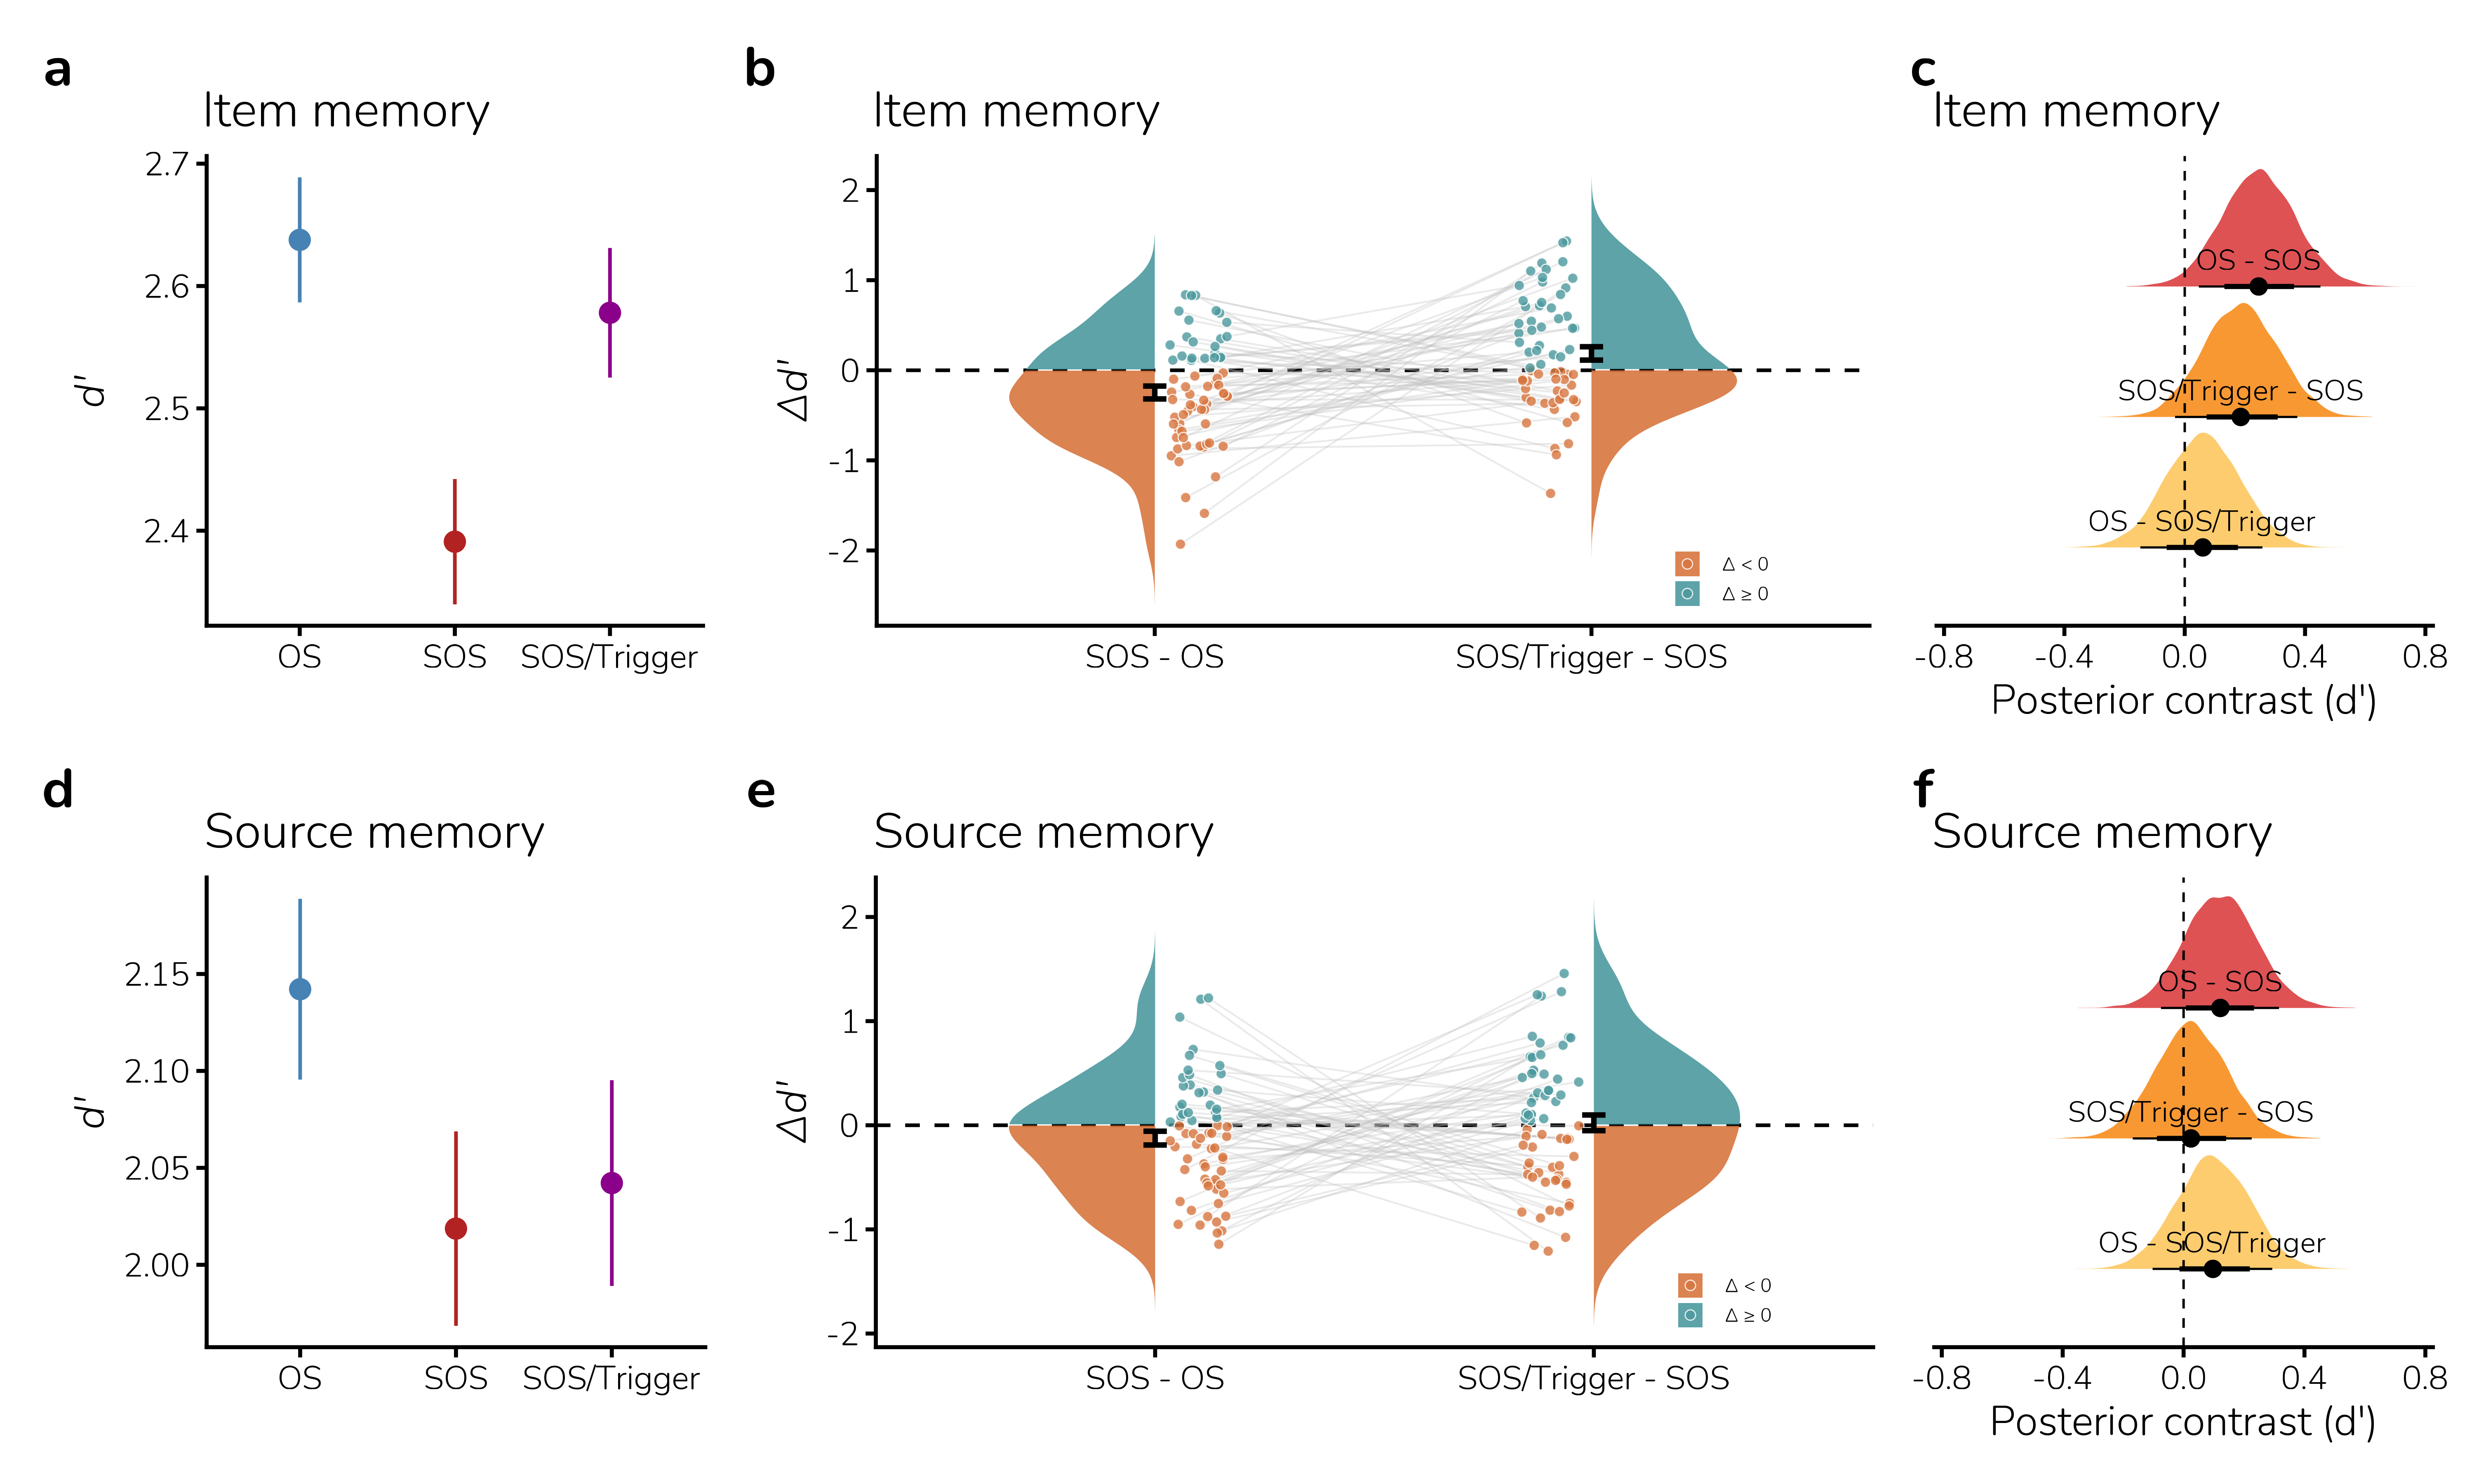
\includegraphics[width=1\linewidth]{figures/closed-loop-fig2.png}
	\caption[Real-time reorienting cues recover item memory but not source memory from pupil-defined arousal-attentional (A-A) suboptimal states (SOS)]{Real-time reorienting cues recover item memory but not source memory from pupil-defined arousal-attentional (A-A) suboptimal states (SOS). SOS and trigger recovery effects for item memory (a,b) and source memory (d,e) \textit{d'}, and estimated marginal contrasts for \textit{d'} (c,f) between the three within-subjects conditions at retrieval. Plots of estimated marginal contrasts show posterior probability distributions. Points indicate posterior medians; thick and thin horizontal lines indicate the 66\% and 90\% HDIs, respectively. Dashed vertical lines mark zero (no difference).}
	\label{fig:closed-loop-fig2}
\end{figure}
\FloatBarrier

\begin{table}[ht!]
	\captionsetup{justification=raggedright,singlelinecheck=off}
	\caption{Six-cell condition matrix.}
	\label{tab:six-cell-matrix}
	\begin{tabular*}{\linewidth}{@{\extracolsep{\fill}}|>{\centering\arraybackslash}m{0.28\linewidth}|>{\centering\arraybackslash}m{0.10\linewidth}|>{\centering\arraybackslash}m{0.18\linewidth}|>{\centering\arraybackslash}m{0.10\linewidth}|>{\centering\arraybackslash}m{0.18\linewidth}|@{}}
		\hline
		\textbf{Original $\downarrow$ Reclassified $\rightarrow$} & \textbf{SOS} & \textbf{SOS-triggered} & \textbf{OS} & \textbf{OS-triggered} \\
		\hline
		\textbf{SOS} & 2011 & 0 & 2466 & 0 \\
		\hline
		\textbf{SOS-triggered} & 0 & 2016 & 0 & 2451 \\
		\hline
		\textbf{OS} & 511 & 0 & 3626 & 0 \\
		\hline
	\end{tabular*}

	\smallskip
	\raggedright
	Six-cell condition matrix crossing real-time pupil-based trial classifications (suboptimal state without trigger, suboptimal state with trigger, optimal state) with drift-corrected reclassifications (suboptimal state without trigger, suboptimal state with trigger, optimal state without trigger, optimal state with trigger).
\end{table}

\subsection{Offline Reclassification Reveals a Continuous Gradient of A-A State Quality}

A fundamental challenge in closed-loop physiological monitoring is the potential for systematic shifts that impact real-time classification algorithms; specifically, pupil measures are susceptible to slow physiological drift (i.e., the ``time-on-task effect") \parencite{unsworth2016pupillary,beatty1982phasic,hopstaken2015multifaceted,martin2022pupillometry,massar2016rewards,steinhauer2022publication,zhao2019pupillometry,schwartz2025eyeris,schwartz2025eyerispaper}. Our primary analysis relied on a causal, real-time pupillometry-based algorithm to detect A-A SOS and deliver visual reorienting cues during the pre-probe fixation period at retrieval on a subset of SOS trials. The real-time algorithm used a fixed baseline computed from the first 20 ``burn-in" trials of each retrieval block to identify subsequent moments when pupil size fell above/below 1 s.d. around the baseline mean. Given that drift can arise from factors such as fatigue, autonomic regulation, and luminance adaptation, to name a few, it is not unreasonable to suspect that within-participant slow trends could impact real-time SOS detection in systematic ways. Critically, use of a fixed early-block baseline (rather than an adaptive rolling baseline, which also has its own challenges) would be impacted by drift such that trials later in the block would be increasingly likely to fall outside the fixed threshold and therefore be classified as SOS trials, even when the participant's A-A state relative to their current physiological baseline has not changed. This design choice, while necessary for real-time implementation in the present study, warrants rigorous post hoc examination.

To validate the robustness of PRISM's SOS detection and to operationalize a continuum of suboptimality, we implemented a post hoc spline drift correction that reclassifies trials independent of slow pupil drift. For each participant and run, we constructed a continuous time series by concatenating the epoched pupil data from the real-time monitoring windows across all trials in trial order, with inter-trial gaps padded with NaN values to preserve the temporal structure of the run (padding duration: 10,416 ms per trial, corresponding to the trigger window, post-trigger fixation, stimulus, and pre-stimulus ITI periods). A natural cubic spline ($df$=5) was then fit to this padded time series using only the non-NaN samples from the real-time monitoring windows, capturing slow non-stationary trends including linear drift and exponential decay components. The spline was evaluated at all timepoints — including the padded intervals — yielding a continuous drift estimate across the full retrieval run (Fig.~\ref{fig:closed-loop-fig3}a). 

\begin{figure}[!tbp]
	\centering
	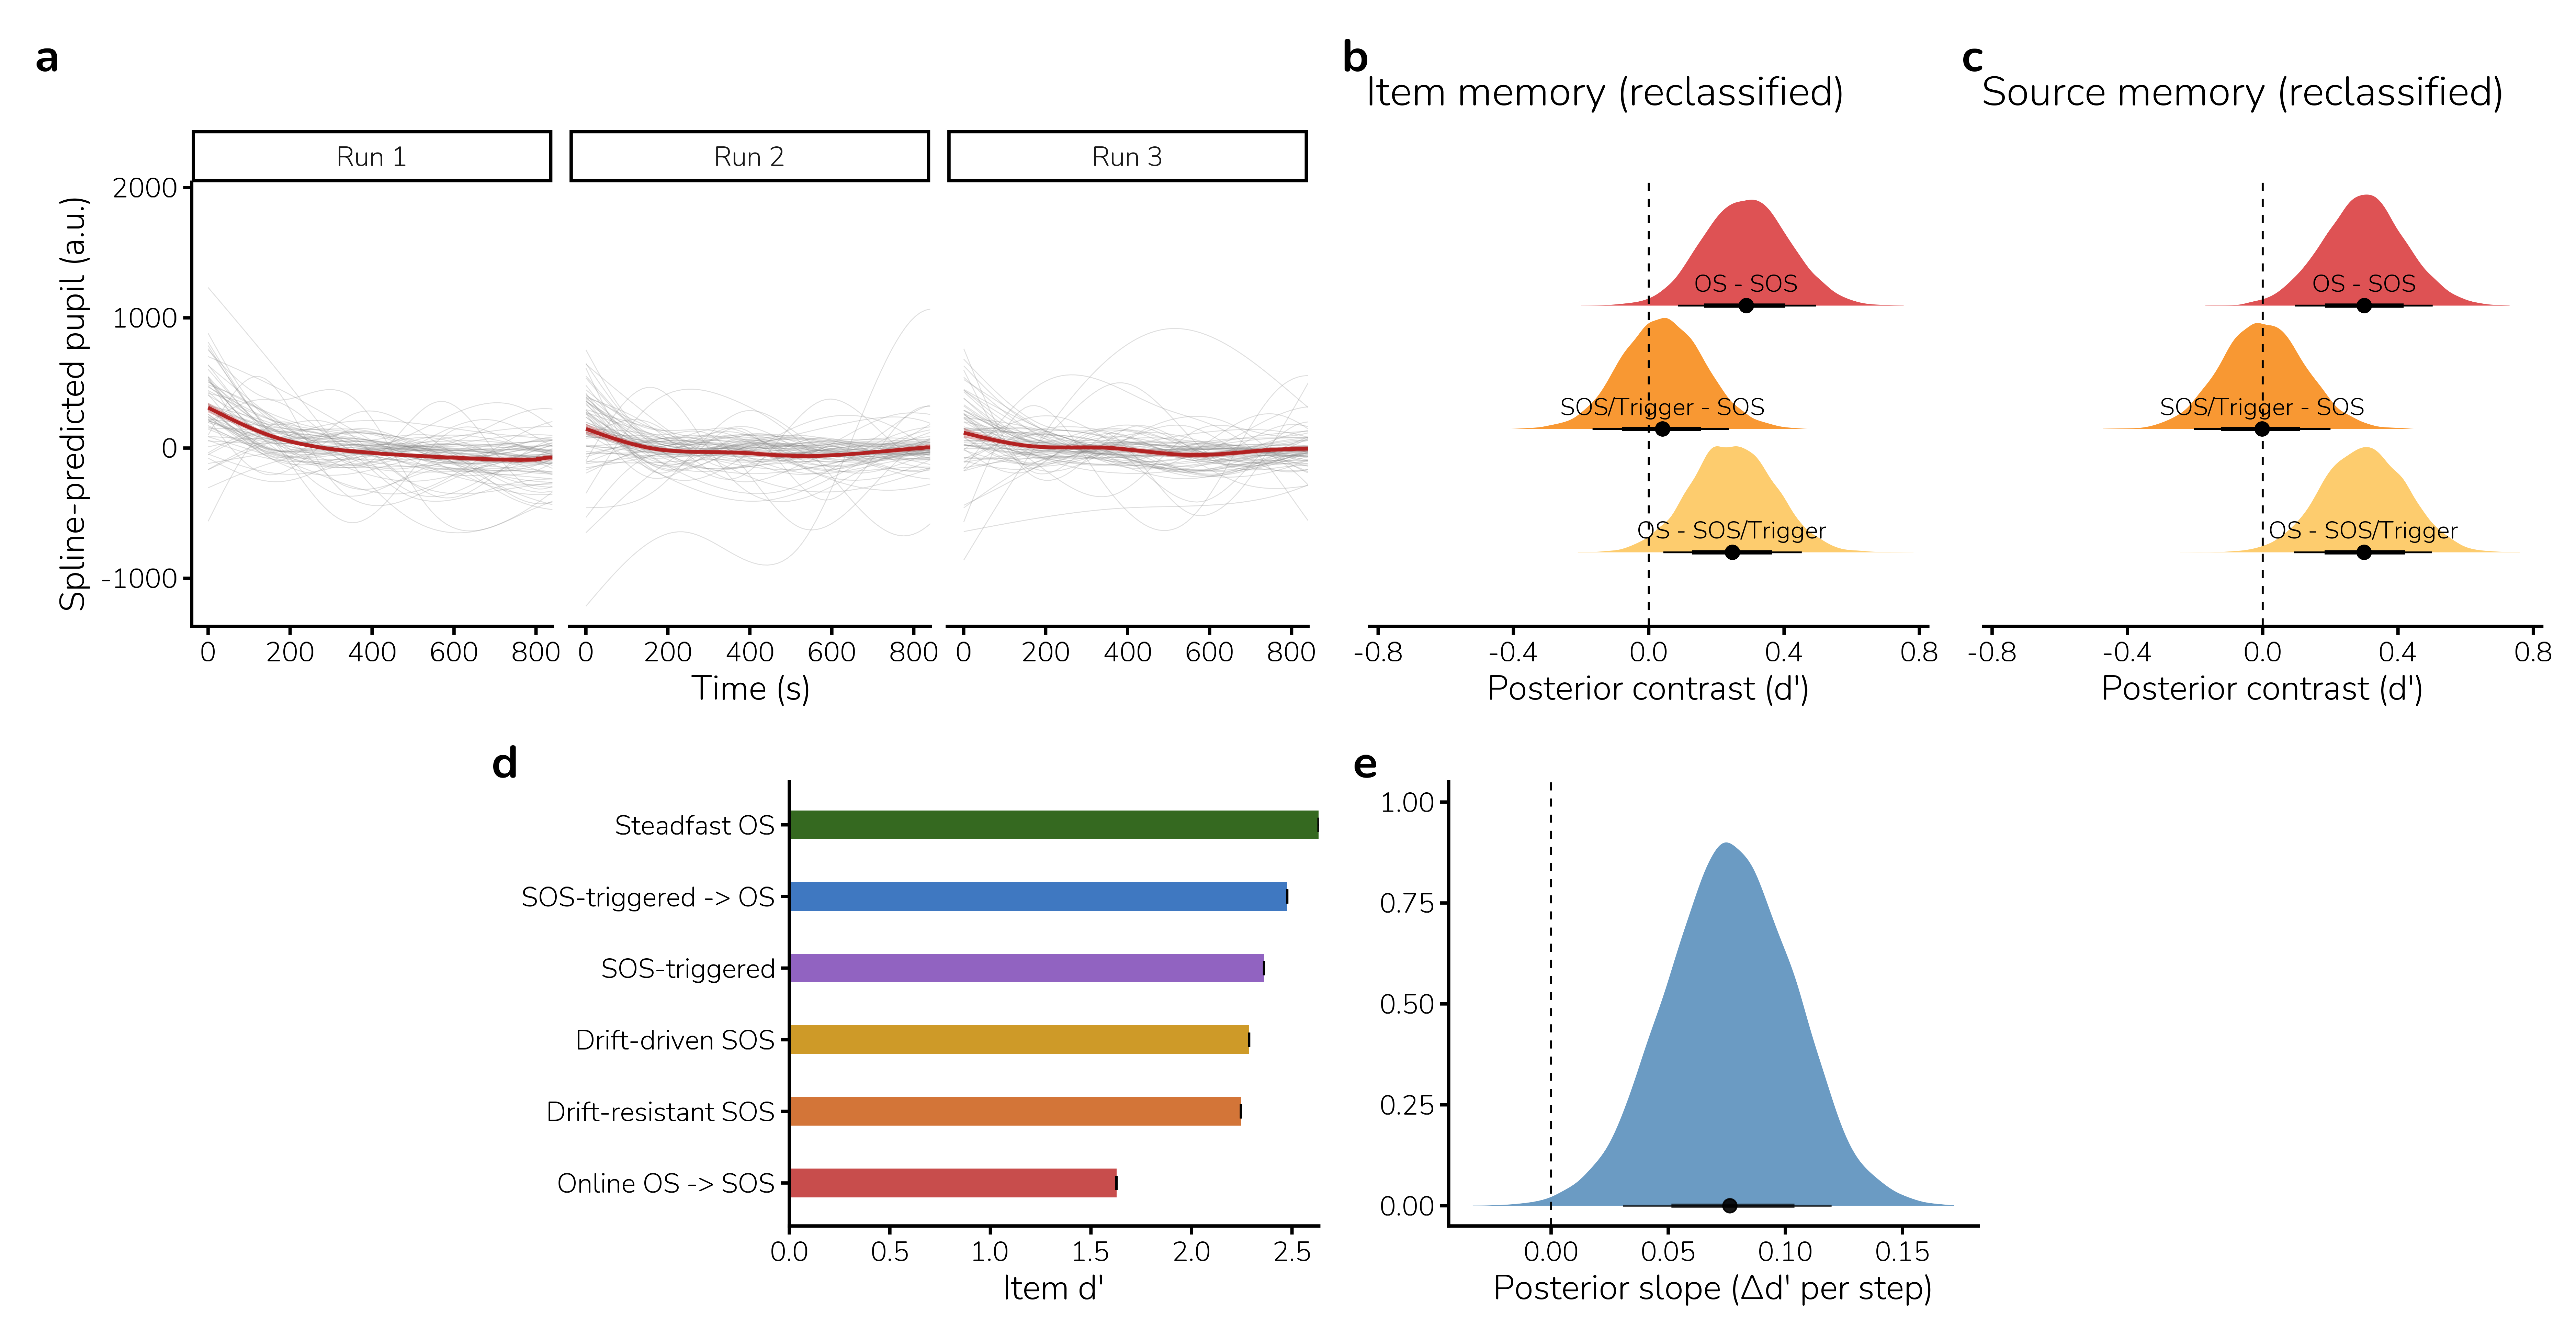
\includegraphics[width=1\linewidth]{figures/closed-loop-fig3.png}
	\caption[Pupil drift characteristics and memory performance after drift-corrected reclassification of arousal-attentional states]{Pupil drift characteristics and memory performance after drift-corrected reclassification of arousal-attentional states. (a) Mean-centered spline-predicted pupil size (arbitrary units) across each of the three experimental runs. Grey lines depict individual participants; the red line and ribbon denote the grand mean $\pm$ 1 s.e.m. Spline fits capture slow, non-stationary drift in the pupil signal that the real-time classification algorithm did not account for. The x-axis is trimmed to 800 s to represent the stable portion of the drift grand mean (as there were varying run lengths per subject — with few spanning beyond 800 s — depending on the number of ``recycled'' trials one encounters in the real-time paradigm). (b,c) Posterior distributions of estimated marginal contrasts for item memory (b) and source memory (c) \textit{d'} between the three within-subjects conditions after drift-corrected reclassification (optimal state, suboptimal state, suboptimal state with trigger). Points indicate posterior medians; thick and thin horizontal lines indicate the 66\% and 90\% HDIs, respectively. Dashed vertical lines mark zero (no difference). (d) Mean item \textit{d'} (log-linear corrected) for each of the six cells of the real-time/reclassified transition table (Table~\ref{tab:six-cell-matrix}). Error bars denote $\pm$ 1 s.e.m. Performance increases monotonically across the four real-time SOS cells (drift-resistant SOS-untriggered, drift-driven SOS-untriggered, drift-resistant SOS-triggered, drift-driven SOS-triggered) to steadfast OS (top). Real-time OS $\rightarrow$ SOS trials (bottom) showed the lowest \textit{d'} of any condition, though this may partly reflect selection artifacts of the spline-based reclassification (see Fig.~\ref{fig:closed-loop-fig4} caption and Discussion). (e) Posterior distribution of the within-subject linear slope fit across the four real-time-SOS cells (drift-resistant SOS-untriggered, drift-driven SOS-untriggered, drift-resistant SOS-triggered, drift-driven SOS-triggered), ordered by inferred depth of suboptimality. The reliably positive slope confirms that drift correction differentiates graded levels of suboptimality among trials that the real-time algorithm uniformly classified as SOS.}
	\label{fig:closed-loop-fig3}
\end{figure}
\FloatBarrier

For each trial, we computed the mean spline prediction during that trial's real-time monitoring window, representing the estimated drift level at the time of that trial. Each trial's monitoring-window pupil mean was then corrected by subtracting the trial-specific spline trend. Unlike the real-time algorithm, which computes thresholds from a baseline initialized over the first 20 burn-in trials, the reclassification thresholds were derived from the global distribution of spline-detrended pupil values across all real-time monitoring samples within the run: trials were classified as SOS if the drift-corrected monitoring-window mean fell above/below 1 s.d. of the global detrended mean. This procedure leverages information from the entire run — including trials that were unavailable to the real-time classifier — providing an alternate drift-corrected reference for threshold computation.

Crossing the real-time and drift-corrected classifications of trials produced a six-cell condition matrix (Table~\ref{tab:six-cell-matrix}). Of the 4,477 real-time SOS-untriggered trials, 2,011 (44.9\%) retained their SOS classification after drift correction — we term these \textit{drift-resistant SOS-untriggered} trials, indicating A-A state departures extreme enough that removing the drift component did not change their classification status. The remaining 2,466 (55.1\%) were reclassified as OS — we term these \textit{drift-driven SOS-untriggered} trials, indicating that their original SOS classification was driven primarily by drift rather than a substantial A-A state departure. Among the 4,467 real-time SOS-triggered trials, 2,016 (45.1\%) remained SOS — we term these \textit{drift-resistant SOS-triggered} trials — and 2,451 (54.9\%) were reclassified as OS — we term these \textit{drift-driven SOS-triggered} trials. Of the 4,137 real-time OS trials, only 511 (12.4\%) were reclassified as SOS after drift correction, representing states where drift had shifted the raw pupil trace toward the baseline mean, masking an underlying suboptimal A-A state that was revealed once drift was removed, while 3,626 (87.6\%) retained their OS classification (i.e., ``steadfast OS trials'').

We then examined whether the observed SOS effect on item and source memory \textit{d'} replicated using the drift-corrected trial reclassification. Under reclassification, there was very strong evidence that item memory \textit{d'} varied with A-A state (OS trials: $m$=2.61, 95\% HPD [2.43, 2.77]; SOS without trigger trials: $m$=2.32, 95\% HPD [2.15, 2.49]; $b$=-0.29, 90\% HDI [-0.50, -0.09], $BF_{10}$=100.69; Fig.~\ref{fig:closed-loop-fig3}b). Source memory \textit{d'} also showed a very strong SOS impairment under reclassification (OS trials: $m$=2.19, 95\% HPD [2.02, 2.36]; SOS without trigger trials: $m$=1.89, 95\% HPD [1.71, 2.06];  $b$=-0.30, 90\% HDI [-0.50, -0.10], $BF_{10}$=121.45) — qualitatively larger than that of the original real-time classification effect (Fig.~\ref{fig:closed-loop-fig3}c).

Next, we examined whether the beneficial trigger effect for item memory observed in the real-time analysis replicated when using the drift-corrected trial classification. When trials were reclassified, the trigger rescue effect on item memory was no longer credible (SOS without trigger trials: $m$=2.32, 95\% HPD [2.15, 2.49]; SOS with trigger trials: $m$=2.36, 95\% HPD [2.19, 2.53]; $b$=0.04, 90\% HDI [-0.16, 0.24], $BF_{10}$=1.69). Source memory similarly showed no trigger rescue (SOS without trigger trials: $m$=1.89, 95\% HPD [1.71, 2.06]; SOS with trigger trials: $m$=1.89, 95\% HPD [1.73, 2.07]; $b$=0.00, 90\% HDI [-0.20, 0.20], $BF_{10}$=0.98). The disappearance of the overall trigger effect under reclassification raises the question of what drives the observed trigger benefit in the real-time data.

\subsection{Item Memory Tracks Depth of Suboptimality Across the A-A State Gradient}

If the drift-corrected classifications capture a meaningful continuum of A-A state quality, then item memory \textit{d'} should vary systematically across the six classification cells. We computed item and source memory \textit{d'}s (log-linear corrected) for each participant for each cell and fit a Bayesian linear model to estimate posterior means and test directed contrasts (see Section~\ref{sec:methods}).

Item \textit{d'} increased monotonically across the four real-time SOS cells –– drift-resistant SOS-untriggered, drift-driven SOS-untriggered, drift-resistant SOS-triggered, drift-driven SOS-triggered –– ordered by inferred depth of suboptimality and trigger delivery (Fig.~\ref{fig:closed-loop-fig3}d). A Bayesian linear slope fit across these four conditions (with a by-participant random intercept) yielded extreme evidence for a positive slope ($b$=0.08, 90\% HDI [0.03, 0.12], $BF_{10}$=351.94), confirming that the drift correction differentiates levels of A-A suboptimality among trials that the real-time algorithm classified as SOS (Fig.~\ref{fig:closed-loop-fig3}e). This gradient was further anchored by the two extreme conditions: real-time OS trials reclassified as SOS trials — i.e., where drift masked suboptimality — showed the lowest \textit{d'} of any condition ($m$=1.63, 95\% HPD [1.45, 1.80]), while steadfast OS trials showed the highest ($m$=2.63, 95\% HPD [2.46, 2.80]).

Unpacking the observed linear slope analysis, for drift-driven SOS trials, which likely fall closer to A-A state optimality than do drift-resistant SOS, the trigger yielded moderate-to-strong evidence of improved item \textit{d'} (drift-driven SOS triggered vs. drift-driven SOS untriggered: $b$=-0.19, 90\% HDI [-0.39, 0.01], $BF_{10}$=15.06). By contrast, for drift-resistant SOS trials, which likely fall further from optimality, the evidence for a trigger-benefit was weaker but directionally consistent (drift-resistent SOS triggered vs. drift-resistent SOS untriggered: $b$=-0.12, 90\% HDI [-0.32, 0.09], $BF_{10}$=4.69). The formal interaction contrasting these two trigger effects was inconclusive ($b$=0.07, 90\% HDI [-0.21, 0.36], $BF_{10}$=2.00), leaving open whether the trigger operates differentially at different depths of suboptimality. Under a fixed-perturbation account — in which a brief A-A-boosting stimulus produces greater functional recovery when the distance to the inverted-U peak is smaller — one would predict a larger trigger benefit for drift-driven than drift-resistant SOS states; the present data are directionally compatible with this prediction but lack the precision to adjudicate it.

Among triggered trials, the severity gradient was partially preserved. Drift-resistant SOS triggered trials showed directionally lower \textit{d'} than drift-driven SOS triggered trials ($b$=-0.11, 90\% HDI [-0.32, 0.09], $BF_{10}$=4.73), though this difference was not credible — consistent with the trigger compressing but not eliminating the gap between adjacent suboptimality levels — in other words, deeply suboptimal states are partially but not fully rescued. The gradient was more clearly evident at the extremes: steadfast OS trials showed credibly higher \textit{d'} than both drift-driven SOS triggered trials ($b$=0.16, 90\% HDI [-0.05, 0.36], $BF_{10}$=8.63) and especially drift-resistant SOS triggered trials ($b$=0.27, 90\% HDI [0.07, 0.47], $BF_{10}$=75.43), indicating that even though the trigger improved item \textit{d'}, performance on triggered SOS trials did not fully recover to the performance level of OS trials.

\subsection{Asymmetric Effects Across Hypo vs. Hyperarousal Suboptimal States}

The inverted-U framework predicts that the trigger's efficacy should depend not only on the magnitude of suboptimality but on its direction; that is, hypoarousal suboptimal states (pupil constriction), which sit on the ascending limb of the inverted-U, should be more amenable to an A-A-boosting intervention than hyperarousal suboptimal states (pupil dilation), which sit on the descending limb where additional arousal might be counterproductive. We tested this by examining the trigger's effect as a function of  whether suboptimality classification was due to pupil constriction or pupil dilation. Among drift-resistant SOS trials (i.e., the most deeply suboptimal states), the trigger credibly improved \textit{d'} for constriction trials ($b$=0.22, 90\% HDI [0.00, 0.43], $BF_{10}$=20.16) but not for dilation trials ($b$=0.03, 90\% HDI [-0.18, 0.24], $BF_{10}$=1.47). The interaction was in the predicted direction, with a numerically larger trigger boost for constrictions than dilations ($b$=0.18, 90\% HDI [-0.12, 0.49], $BF_{10}$=5.24). Expanding to all SOS trials (both drift-resistant and drift-driven) to increase statistical power, the pattern held (constriction trigger boost: $b$=0.18, 90\% HDI [-0.04, 0.40], $BF_{10}$=10.87; dilation trigger boost: $b$=0.06, 90\% HDI [-0.17, 0.28], $BF_{10}$=1.97). This asymmetry is consistent with the prediction that suboptimality is not sign-neutral with respect to recovery in that a brief A-A-boosting cue can nudge low-A-A states toward the inverted-U peak, but the same perturbation is less effective — or potentially counterproductive — for states that are already at the high-A-A extreme. However, among drift-driven SOS trials (i.e., the marginally suboptimal states nearer to the peak) the trigger boost did not credibly differ between constrictions and dilations (constriction: $b$=0.03, 90\% HDI [-0.23, 0.29], $BF_{10}$=1.42; dilation: $b$=0.00, 90\% HDI [-0.27, 0.26] $BF_{10}$=0.96; interaction: $b$=0.04, 90\% HDI [-0.34, 0.42], $BF_{10}$=1.30), which suggests that trials that fall modestly away from optimality can benefit from A-A cuing. An interesting open question is whether the effect of the cue is due to increasing arousal and attention for such trials in the hypo-A-A arm but perhaps due solely to increasing attention (without adverse further increases in arousal) in the hyper-A-A arm.

\begin{figure}[!tbp]
	\centering
	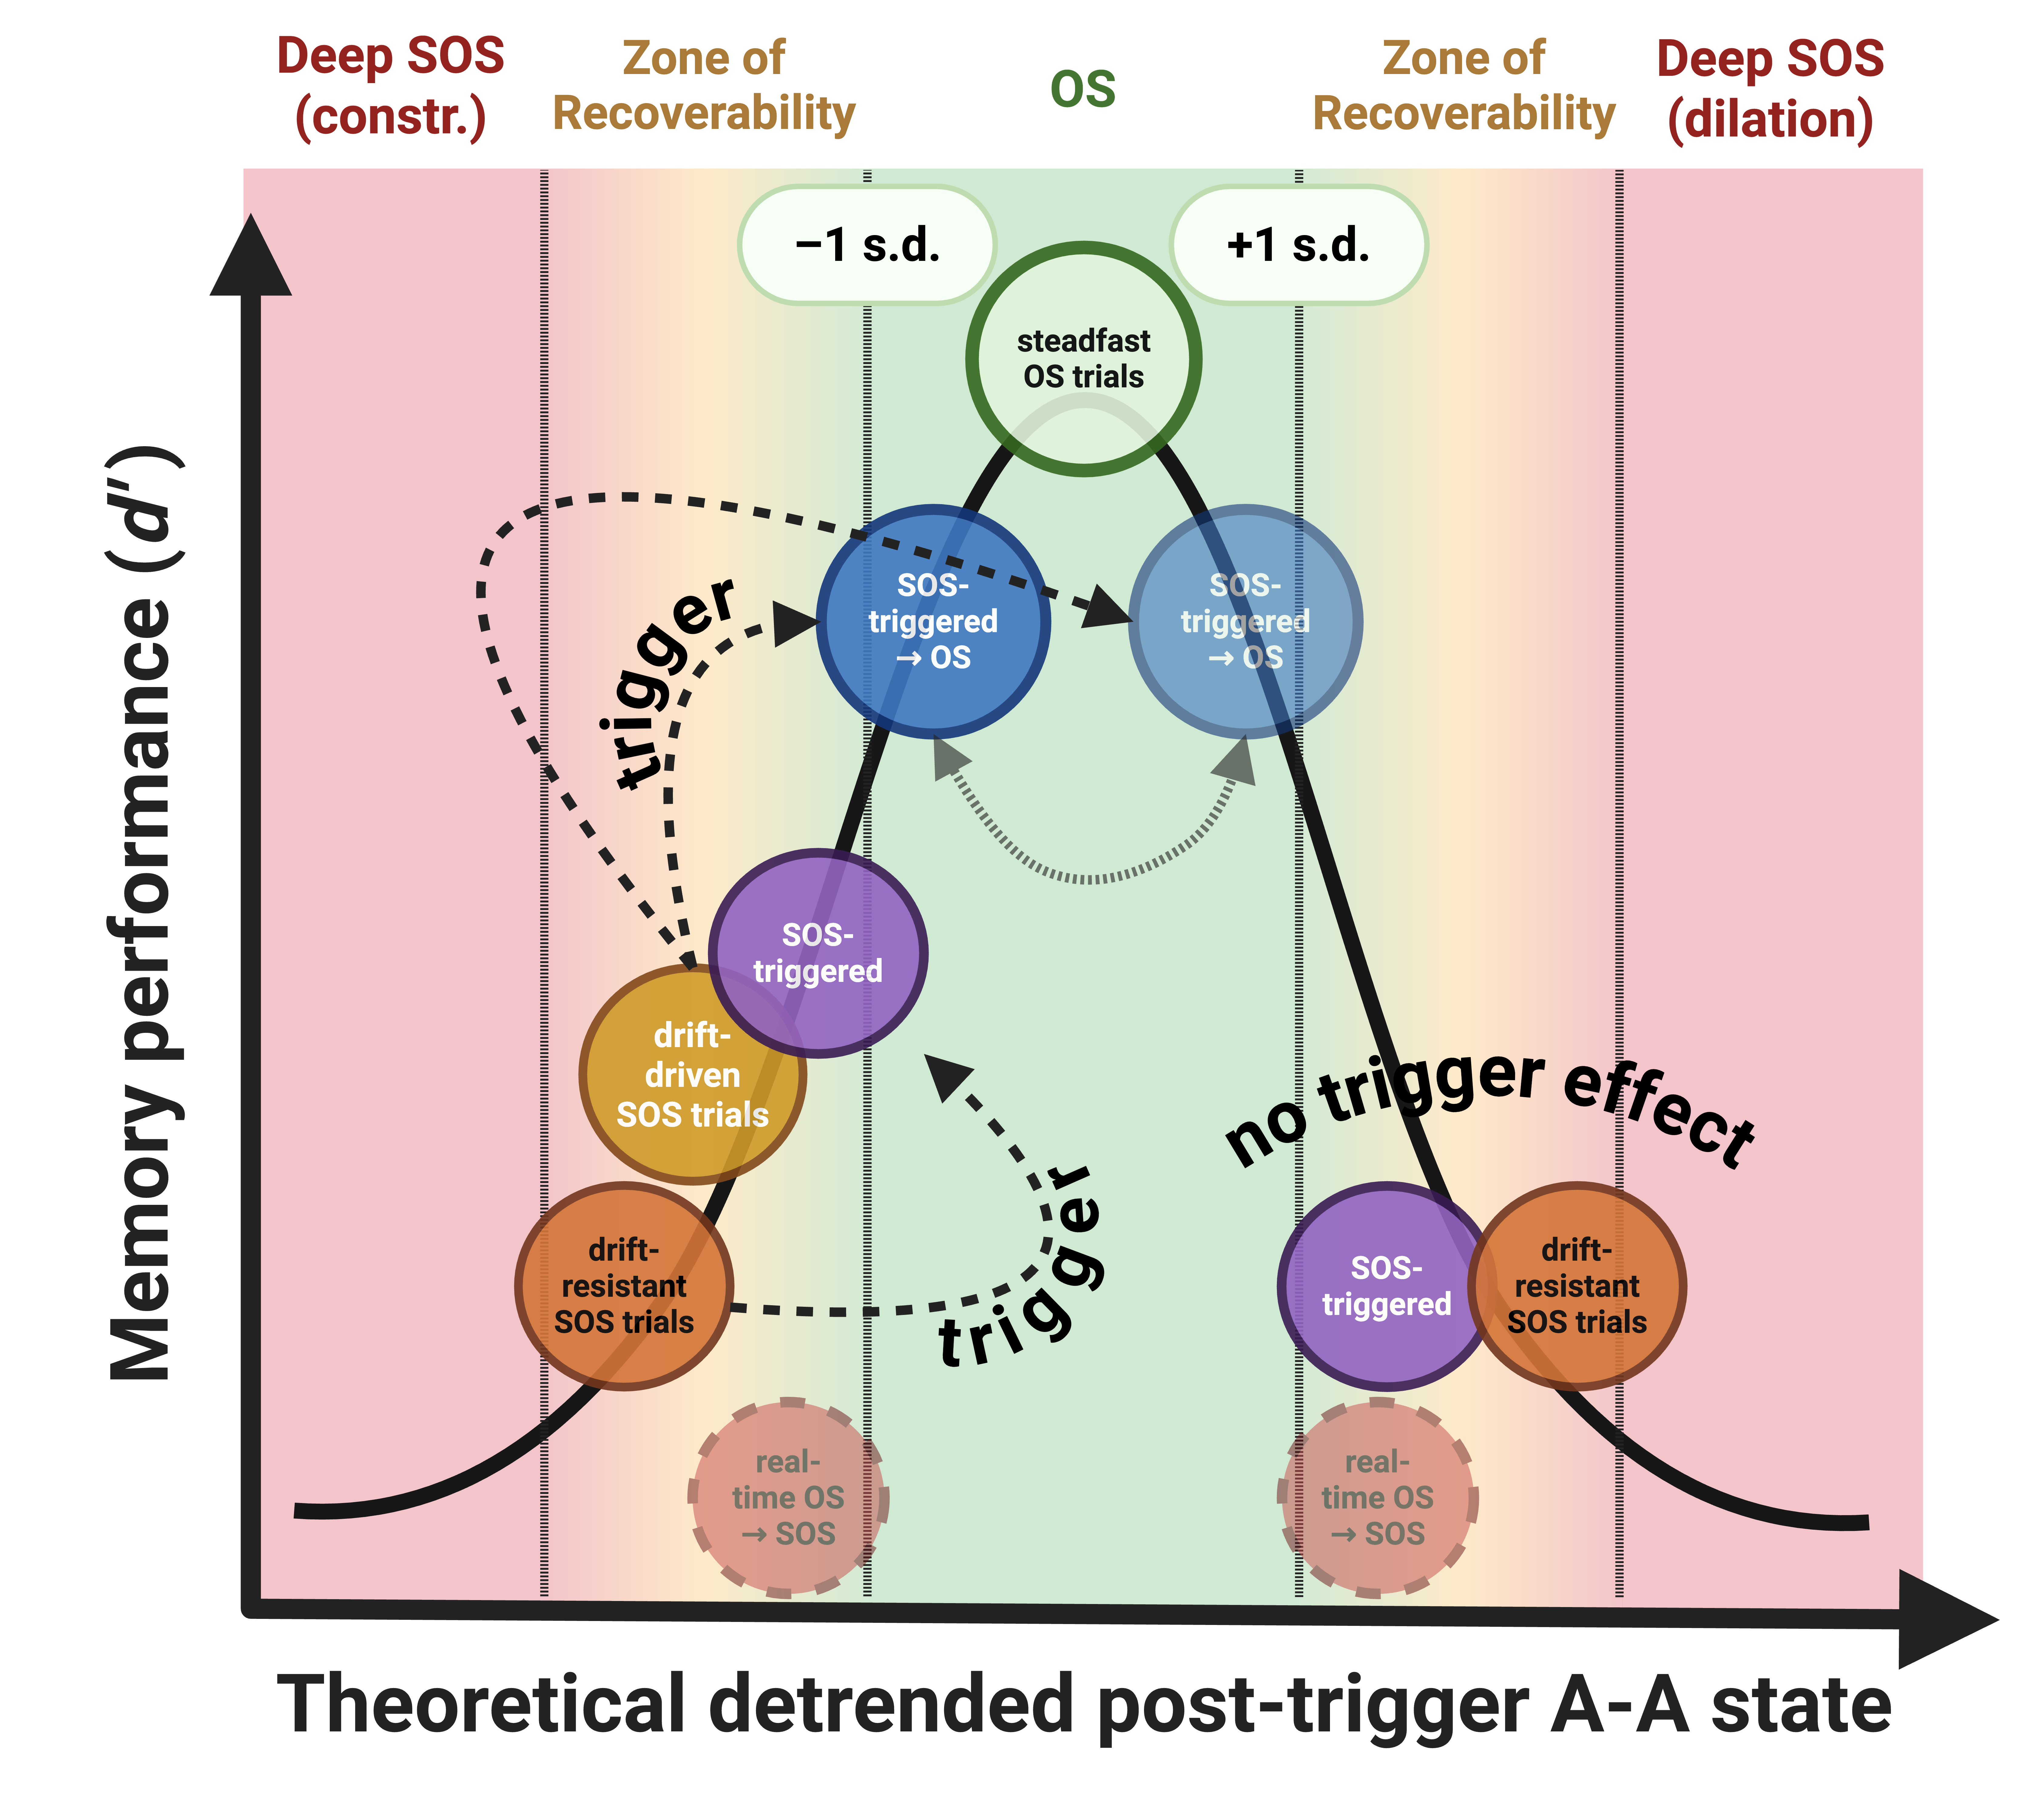
\includegraphics[width=0.6\linewidth]{figures/closed-loop-fig4.jpg}
	\caption[Theoretical framework mapping drift-corrected trial classifications onto an inverted-U shaped arousal-attentional (A-A) state continuum and their predicted memory performance]{Theoretical framework mapping drift-corrected trial classifications onto an inverted-U shaped arousal-attentional (A-A) state continuum and their predicted memory performance. The x-axis represents the theoretical detrended post-trigger A-A state, ranging from deep suboptimal states (SOS) driven by pupil constriction (left) to deep SOS driven by pupil dilation (right), with the optimal state (OS) zone at center (bounded by $\pm$1 s.d.). The y-axis represents memory performance (item \textit{d'}). The solid black curve depicts the predicted inverted-U relationship between detrended A-A state and memory performance. The six trial categories from the drift-corrected reclassification are positioned according to their inferred A-A states. Drift-resistant SOS trials (orange circles) occupy both deep SOS extremes, reflecting A-A departures severe enough to survive drift correction. Drift-driven SOS trials (yellow circle) fall within the Zone of Recoverability on the constriction side, indicating that their original SOS classification was attributable primarily to drift rather than a putative A-A state departure. SOS-triggered trials that remained SOS after drift correction (purple circles) appear at both extremes, whereas SOS-triggered trials reclassified as OS (blue circles) sit within or near the OS boundary on both sides. Steadfast OS trials (green circle) occupy the center of the OS zone. Real-time OS $\rightarrow$ SOS trials (faded red circles) are depicted off the inverted-U curve to reflect that their position along the A-A state continuum does not conform to the predicted mapping. Although these trials exhibited the lowest \textit{d'} of any condition, their mean detrended pupil deviations were closer to zero than those of the drift-resistant SOS trials, placing them nearer to the OS zone rather than at the deep SOS extremes. This discrepancy likely arises from a selection bias inherent to spline-based reclassification: OS $\rightarrow$ SOS reclassification requires that the spline trend shifted away from the real-time baseline, and trials on the same side as this shift are mechanically constrained to be closer to the corrected mean than trials whose optimality status survived correction. The reduced opacity and placement below the curve further reflect the instability of \textit{d'} estimates for this condition due to low trial counts (511 total trials across all subjects). Dashed arrows illustrate the effect of the reorienting cue, which elevates performance for trials within the Zones of Recoverability but has no effect on trials in the deep SOS dilatory extreme, where the A-A state departure is too severe for a brief visual reorienting cue to remediate.}
	\label{fig:closed-loop-fig4}
\end{figure}
\FloatBarrier

\section{Discussion}

Multiple neurocognitive processes influence whether and how humans remember or forget, including preparatory processes that render certain moments more conducive to successful retrieval than others. The present study provides further evidence that pupil-indexed suboptimal arousal/attentional states at retrieval are associated with impaired item recognition and source recollection \parencite{robison2022pupillary,madore2022readiness,madore2020memory}, and provides novel evidence that a real-time A-A intervention just prior to an attempt to remember can rescue item recognition memory. Because the trigger manipulation occurred exclusively at retrieval — following each encoding period — these results provide causal evidence that phasic reorienting during A-A-defined suboptimal states affects item recognition at the retrieval stage, independent of encoding quality. These findings illustrate how a closed-loop pupillometry paradigm with phasic reorienting during arousal/attentional suboptimal states can causally improve memory access, extending the readiness-to-remember framework from correlational observation to real-time intervention. We discuss the implications of the present findings for theory and application.

\subsection{Hippocampal and Cortical Retrieval Mechanisms}

The observed rescue of item memory but not source memory, combined with the observation that the trigger effect was significantly larger on item \textit{d'} than on source \textit{d'}, bears on theories of episodic retrieval. Dual-process models of recognition memory distinguish between familiarity — a rapid signal indexing item memory strength — and recollection — a slower, controlled process that recovers specific episodic details such as the encoding context. Extant data suggest that, relative to familiarity, recollection is more disrupted by division of attention at the time of retrieval and is differentially dependent on hippocampal pattern completion, with the latter being influenced by LC-NE arousal and attentional modulatory input. Familiarity-based item recognition decisions can be affected by division of attention, though to a lesser extent than recollection, and differentially depend on medial temporal cortical computations. While goal-directed attentional gain signals can increase familiarity, the influence of LC-NE arousal and attentional modulatory input on familiarity remains unclear.

The item recognition decisions in the present study may reflect familiarity-based memory in the absence of recollection or a mix of familiarity-based memory with and without non-criterial recollection (i.e., recollection of other encoding features beyond source details). The selective rescue of item memory, in the absence of a corresponding benefit for source memory, aligns with the dual-process view that familiarity and recollection rely on partially distinct neural substrates. We speculate that, in the current study, the reorienting trigger promoted an increase in arousal and a phasic reallocation of visuospatial attention to the location where the retrieval probe would appear, increasing neural gain and thus boosting the strength of medial temporal cortex familiarity elicited by the retrieval probe. Future studies are required to determine whether these effects are due to gain amplification of cortical signals that project to perirhinal and/or parahippocampal cortical structures from which familiarity signals emerge as well as whether such amplification is due to LC-NE modulatory effects or to effects of visuospatial attention.

By contrast, the phasic arousal and attentional reorienting elicited by the brief trigger was insufficient to increase the sustained, goal-directed attentional state needed to boost recollection-based memory decisions. It may be the case that a more sustained or semantically targeted reorienting cue is needed to facilitate recollection during suboptimal A-A states. Future work could test this prediction by comparing reorienting cues of varying duration, complexity, and/or semantic content — for example, reinstating the encoding goal cue itself — to determine whether richer interventions can additionally rescue source recollection.

\subsection{Intervening Across the Arousal/Attentional State Continuum}

The present drift-corrected reclassification analysis offers a window into the heterogeneous nature of A-A suboptimal states and potential boundary conditions of real-time intervention. A key insight from the reclassification analysis is that the trials originally classified as SOS by the real-time algorithm fall along a continuum of A-A state deviation severity, ranging from threshold-proximal SOS –– in which pupil-indexed arousal/attention deviates only slightly beyond the detection threshold — to deep SOS — in which states deviate substantially from the participant's current physiological baseline, reflecting a more profound deviation from LC-NE tone optimality in the moment immediately preceding a retrieval trial.

This distinction provides an account of the pattern of results observed under reclassification. The conservative spline-correction procedure, by removing slow drift and recomputing global thresholds against the full session baseline, effectively partitions the original SOS trials into these two categories. Trials that remain classified as SOS under both the real-time and drift-corrected methods represent deep SOS: A-A state deviations that are robust to the choice of baseline and detrending method. Among these deep SOS, the trigger conferred a weaker and less certain memory benefit than among drift-driven SOS trials ($BF_{10}$=4.69), suggesting that when arousal/attention has deviated further from the optimal zone, a brief visual flickering cue may be insufficient to restore the preparatory state needed for successful memory retrieval.

By contrast, the approximately 55\% of original SOS trials that were reclassified as OS by the drift-correction method represent threshold-proximal SOS — trials on which the real-time algorithm detected a threshold crossing, but the deviation was mild enough that, once slow drift is accounted for, these trials fall within the normal range of A-A state fluctuation. It is among these threshold-proximal SOS trials that the clearest trigger benefit emerged: trials that received the reorienting cue showed moderate-to-strong evidence of higher item memory than those that did not ($BF_{10}$=15.06). This pattern is consistent with the view that threshold-proximal A-A state deviations occupy a \textit{zone of recoverability}; the arousal/attention system has drifted from optimal but has not disengaged or overengaged so deeply that a phasic reorienting signal cannot pull it back. Here, the brief visual trigger, by evoking a transient LC-NE-mediated phasic response and/or increase in visuospatial attention, appears sufficient to nudge the system from a mildly suboptimal state back toward the A-A threshold necessary for successful memory expression.

Taken together, this framing reinterprets the disappearance of the trigger benefit under drift-corrected reclassification not as evidence against the efficacy of real-time intervention, but as suggestive of a dose-response relationship between SOS severity and intervention efficacy. Indeed, the trigger produced directionally consistent benefits at both levels of reclassified suboptimality, and the pattern of simple effects — a stronger trigger benefit for drift-driven than drift-resistant SOS trials — is consistent with a fixed-perturbation account in which a brief arousal/attentional-boosting stimulus yields greater functional recovery when the distance to the inverted-U peak is smaller. However, the formal interaction contrasting these two trigger effects was inconclusive ($BF_{10}$=2.00), and the present data lack the precision to definitively establish that the trigger operates differentially at different depths of suboptimality. The depth-of-suboptimality interpretation therefore rests on the converging pattern of simple effects and the monotonic linear increase in item \textit{d'} across the four real-time-SOS cells ($BF_{10}$=351.94), rather than on a credible interaction. Future studies with larger samples or adaptive designs that oversample deep SOS trials could provide the statistical precision needed to formally adjudicate this question.

Notably, while item \textit{d'} varied across the six reclassified cells ordered by inferred depth of suboptimality — anchored by deep SOS trials at the bottom and steadfast OS trials at the top — the within-real-time-SOS comparison between drift-resistant and drift-driven untriggered trials did not yield a credible difference in \textit{d'} ($BF_{10}$=1.70). If drift correction captures a meaningful severity gradient, one might expect drift-resistant trials to show detectably lower \textit{d'} than drift-driven trials. Two considerations temper this concern. First, per-subject cell sizes for these conditions are modest, limiting sensitivity to detect what may be a small difference between neighboring points on the continuum. Second, the performance function may be relatively flat across the mildly-to-moderately suboptimal range and steepen only at the extremes — a pattern that would produce the observed result in which the broad reclassified-SOS vs. reclassified-OS contrast is large but the within-SOS gradient is undetectable at our sample size. Importantly, the evidence for graded suboptimality does not depend solely on \textit{d'} differences between drift-resistant and drift-driven cells; it is supported by the monotonic slope across the four real-time-SOS cells, by the differential trigger effects across those cells, and by the constriction/dilation asymmetry reported below.

\subsection{Intervening Across Hypo- and Hyper- Arousal/Attentional States}

Among drift-resistant SOS trials (i.e., the most deeply suboptimal states), the trigger credibly improved \textit{d'} for constriction trials ($BF_{10}$=20.16) but not for dilation trials ($BF_{10}$=1.47), with the interaction directionally favoring constrictions ($BF_{10}$=5.24) though not reaching conventional credibility thresholds. This pattern is consistent with the inverted-U framework's prediction that hypoarousal states, situated on the ascending limb, are amenable to an A-A-boosting intervention that shifts the system toward optimality, whereas hyperarousal states, situated on the descending limb, should not benefit from — and may even be harmed by — additional arousal/attention. Moreover, this asymmetry was absent among drift-driven SOS trials (all $BF_{10}$\textless1.5), which suggests that the differential effects of intervention may depend on whether suboptimality is far from vs closer to the peak of the inverted-U curve. While only suggestive, this pattern may inform future closed-loop interventions: Adaptive algorithms that detect the direction of the A-A departure could, in principle, deploy different intervention strategies for hypoarousal A-A versus hyperarousal A-A states depending on the degree of suboptimality — for instance, an alerting cue for extreme pupillary constrictions and a calming or refocusing cue for extreme pupillary dilations, whereas a common approach may suffice for state deviations closer to optimality.

\subsection{Limitations and Future Directions}

Several limitations of the present study warrant consideration. First, our real-time SOS detection relied on a fixed early-block baseline, which, as the spline-detrending analysis revealed, is susceptible to slow physiological drift. While the reclassification analysis demonstrated that the core findings are robust to this limitation, future implementations of PRISM could incorporate adaptive, rolling baseline algorithms that are less sensitive to low-frequency drift while remaining causal. Second, the reorienting trigger was a simple visual flicker — a low-level, non-semantic cue that may have boosted arousal, visuospatial attention, or both. While this design choice enabled experimental control by holding the cue constant across all triggered trials, it also limits mechanistic understanding of the trigger effect, as well as the ecological validity and potential potency of the intervention. Real-world applications might benefit from more targeted cues, such as brief reminders of the task goal or multi-sensory stimulation, which could potentially rescue both item and source memory. Third, although the within-subject design controls for many individual differences, participants varied considerably in their SOS rates and trigger responsiveness. Characterizing the individual difference factors that moderate closed-loop intervention efficacy — including trait-level sustained attention capacity, working memory, and baseline autonomic arousal/attention — remains an important direction for future real-time research. Fourth, while pupil size provides a continuous, non-invasive index of central arousal/attention, it is an indirect and non-specific measure. Pupil dynamics reflect contributions from multiple ascending neuromodulatory systems --- including the LC-NE system, cholinergic projections from the basal forebrain \parencite{reimer2016pupil}, and broader autonomic input --- as well as several non-cognitive factors (e.g., luminance, fatigue). The framing of pupil-indexed suboptimal states in this chapter as reflecting LC-NE--mediated arousal/attention should therefore be read as one motivating hypothesis rather than a tested mechanism. The present design demonstrates that pupil-defined preparatory states causally affect retrieval, but it does not adjudicate among the neuromodulatory systems that contribute to those pupil dynamics. Future work coupling pupillometry with simultaneous measures sensitive to specific neuromodulatory contributions --- for example, concurrent pupillometry with EEG, with high-resolution functional MRI, or with pharmacological challenges that selectively perturb noradrenergic vs.\ cholinergic tone --- would help dissociate these systems' contributions to the observed effects. Finally, the present study focuses on young adult participants with normal vision and no neurological disorders; the translational potential of PRISM for clinical populations with attentional dysregulation — such as individuals with ADHD, traumatic brain injury, and/or age-related cognitive decline — represents a promising but untested avenue.

In summary, the present study demonstrates that real-time detection of and intervention on arousal-attentional suboptimal states immediately preceding attempts to remember can causally rescue item memory performance, providing closed-loop pupillometry evidence for the readiness-to-remember framework. The distinction between item and source memory rescue suggests that a brief reorienting cue is sufficient to boost familiarity-based recognition but not recollection of the encoding context. The spline-detrending reclassification reveals that the trigger's efficacy varies with the depth of suboptimality, emerging most clearly for marginally suboptimal states within a zone of recoverability, and that its direction matters in that hypoarousal/attentional states on the ascending limb of the inverted-U are more amenable to an A-A-boosting intervention than are hyperarousal/attentional states on the descending limb. Together, these findings advance understanding of how moment-to-moment fluctuations in arousal and attention influence the expression of episodic memories, and they establish a framework that tailors real-time intervention to both the severity and direction of arousal-attentional departure from optimality, with implications for educational practice, clinical intervention, and the design of adaptive cognitive technologies that seek to optimize human cognitive performance in real time.

\section{Materials and Methods}\label{sec:methods}

\subsection{Participants}

Seventy-nine participants were enrolled in the study (54 female participants; $m_{age}=21.73$ years, $s.d.=1.92$, $range=18–25$ years), based on sample sizes used in similar studies \parencite{madore2020memory}. Participants were recruited from print and online advertisements at Stanford University and the surrounding community, were all native English speakers, reported not concurrently participating in any other study or in any study with contraindications to the primary hypotheses of the current study, reported no known neurological impairment, history of seizures and/or photosensitive epilepsy, nor severe dizziness, vertigo, and/or motion sickness, and did not possess an implanted pacemaker or defibrillator. All participants self-reported normal or corrected-to-normal vision, no known colorblindness, and normal or corrected-to-normal hearing in addition to passing a standardized vision test (ZEISS Online Vision Screening; \url{https://visionscreening.zeiss.com/en-US}), which included tests of visual acuity, contrast vision, color vision, and signs of astigmatism. All participants provided written informed consent and were compensated US\$20 per hour, in accordance with procedures approved by Stanford's Institutional Review Board. Data from 10 participants were excluded for the following reasons: (a) five participants were excluded from analyses owing to too few lapsing trials; (b) another two participants for too many lapsing trials (i.e., exceeding 2 s.d. of the mean proportion of lapsing trials relative to all participants); (c) one participant was excluded for having source \textit{d'} less than or equal to zero; and (d) two participants were excluded from the study owing to failure to comply with task instructions. Two participants withdrew from the study altogether. Thus, data from 67 participants were retained for all analytics.

\subsection{Experimental Design}

Participants completed a 2.5-h session: set-up, vision test, and task instructions (30 min), goal-directed encoding and retrieval phases (1.5 h) and a separate individual differences assessment (30 min). Only the memory task included pupillometry measurements. Key components of the memory task (design, goal states, and common object pictures) were adapted from prior research that demonstrated the behavioral and functional neural correlates of item and source memory retrieval goals \parencite{dobbins2005domain}. The individual differences assessment was adapted from a prior study linking preparatory attention to item and source memory performance \parencite{madore2020memory}), and comprised two task-based assays of sustained attention — the gradual-onset continuous performance task (gradCPT) \parencite{esterman2013zone} and the sustained attention to response task (SART) \parencite{debettencourt2019realtime} — as well as self-report questionnaires probing measures of media multitasking, spontaneous mind wandering, attention-deficit/hyperactivity disorder (ADHD) and attentional impulsivity. The present manuscript focuses on within-participant effects; thus, these individual-difference assays are not reported herein.

\subsection{Goal-Directed Encoding and Source Memory Retrieval Task}

All tasks were run using custom PsychoPy scripts in Python \parencite{peirce2007psychopy}. The fixation cross, goal cue, and object on each trial were presented centrally on a white background screen and were luminance- and chrominance-controlled and matched using the SHINE toolbox in MATLAB \parencite{willenbockel2010controlling,dalben2023shine}. Stimuli were presented on a Mitsubishi Diamond Pro 2070SB SuperBright Diamondtron cathode-ray tube display (June 2004 model) to ensure that low-level visual properties did not affect pupillary assays. The display was 40 cm wide $\times$ 30 cm tall at a resolution of 1024$\times$768 px, where 400 px is approximately 15.6 cm. Participants' eyes were situated approximately 50 cm from the monitor and performed the task in a stabilizing head- and chin-rest. A 5-point eye-tracker position calibration and validation procedure was performed prior to each run. All participants were run in the same testing environment –– a dimly lit room in which the only light sources were the stimulus display and a dim floor lamp situated approximately 3 ft behind the participant; no fluorescent overhead lights were used during the session.

\subsubsection{Encoding}

Participants viewed 168 objects once across three intentional encoding runs (7 min 56 s per run) of 56 trials each. Each encoding phase run preceded its corresponding retrieval phase run. On each trial (Fig.~\ref{fig:closed-loop-fig1}a), a fixation cross appeared for 4.0 s, followed by one of two possible task orienting goal cues ('pleasant or unpleasant'; 'bigger or smaller') for 1.6 s; a 0.1-s goal cue to stimulus interval was then followed by an object for 2.8 s. To minimize eye-gaze related pupillary artifacts, participants were instructed to keep their eyes fixated on the fixation cross until the goal cue or object appeared. Participants performed object classification based on a conceptual goal (does the object evoke feelings of pleasantness or unpleasantness) or a perceptual goal (is the object physically bigger or smaller in size on the screen, irrespective of real-world size), responding as quickly and as accurately as possible. Participants made each judgment with one of two button presses (pleasant or unpleasant; bigger or smaller) on a Sony PlayStation 5 DualSense® Wireless Controller using their right thumb ($\square$ button to respond `pleasant' or `bigger', $\bigcirc$ button to respond `unpleasant' or `smaller'). Participants received detailed verbal and visual instructions from the experimenter and were frequently given the opportunity to ask clarifying questions before moving on to the next instruction. There were eight interactive practice trials to ensure task comprehension before moving on to the real task runs. Interactive practice was monitored closely by the experimenter and repeated until the participant demonstrated clear understanding of the task instructions and controller button-to-response mapping, typically occurring following the first or second round of practice trials.

In each encoding run, 28 objects were classified on the conceptual goal dimension (pleasant or unpleasant) and 28 on the perceptual dimension (bigger or smaller), yielding 84 conceptual object trials and 84 perceptual trials across runs. Each object appeared either bigger (450$\times$450 px) or smaller (150$\times$150 px) in size on the screen, independent of goal cue, counterbalanced across participants through random assignment. Thus, objects were crossed in a 2$\times$2 design, with 14 objects from each size crossing ('pleasant or unpleasant?' and bigger, `pleasant or unpleasant?' and smaller, `bigger or smaller?' and bigger, and `bigger or smaller?' and smaller) appearing in a random order per run (with the constraint that a particular goal –– for example, `pleasant or unpleasant' –– could not appear more than four times consecutively). Thus, each participant received a random assignment of 168 goal-object pairings at encoding.

\subsubsection{Retrieval}

Following each encoding run, all participants were given a 5-min interphase rest period and were permitted to stand up, stretch, walk around the dimly lit room, and/or sit back and close their eyes. During this interphase retention interval, participants were also played a medley of relaxing music. Following the interphase period, participants performed a retrieval phase for objects from that immediately preceding encoding block. Specifically, at retrieval, they viewed 84 objects –– 56 studied and 28 novel foils –– across each of three goal-directed retrieval runs of 84 trials each (252 total objects). Similar to the encoding phase, objects appeared in a random order per run (with the constraint that an object's associated encoding phase goal –– for example, `pleasant or unpleasant' –– could not appear more than three times consecutively).

Participants were instructed that in each retrieval run, medium-sized versions of objects from the immediately preceding encoding phase run would be intermixed with new objects that they have never seen before in the experiment. On each retrieval trial, participants made a four-alternative forced-choice (4-AFC) memory judgment on each medium-sized test object (300$\times$300 px), wherein they decided whether they: (1) remember having performed the size decision task (i.e., bigger or smaller before) with the object at encoding, (2) remember having performed the pleasantness decision task (i.e., pleasant or unpleasant before) with the object at encoding, (3) remember having encountered the object at encoding, but cannot remember which decision task was performed, or (4) do not remember having encountered the object and thus perceive it as new. 

Each retrieval trial (Fig.~\ref{fig:closed-loop-fig1}b) began with a 4-s intertrial interval (ITI) consisting of a fixation cross. The final 2 s of this interval –– for the first 20 trials of each retrieval run –– constituted the relevant analytic window for ``burn-in'' trials to establish robust baseline pupillometry metrics before threshold-based assessment of A-A states and, on a subset of trials, triggering commenced. Beginning on trial 21, following the 4-s ITI, real-time pupillometry was conducted across either one or two 1-s real-time sampling windows to assess momentary pupil dilation (note that if a SOS was not detected in the first 1-s window the second 1-s window was assessed, which provided more opportunities for detection of a SOS and then, on a subset of trials, real-time triggering). A second 1-s sampling window also appeared when the first 1-s window contained excessive missing pupil data (pre-determined to be $\geq$20\% of pupil samples). Data from each real-time window then underwent real-time blink padding (100 ms) and linear interpolation; if more than 50\% of the real-time time series following blink padding were missing values, the real-time window sample was rejected. Moreover, we implemented a real-time trial recovery approach to increase power by reducing the number of trials with no reliable real-time triggering data; here, we ``recycled'' trials if both 1-s real-time sampling windows were impacted by excessive missing pupil data. Recycling consisted of displaying a control probe (a luminance-matched gray-tan circle with a radius of 150 px, the color of which was determined by averaging the RGB values for all possible object probe stimuli) in lieu of an object probe, and the trial was restarted for up to three additional repetitions (totaling up to four possible trial initiations per object) before marking real-time data for that object unusable. Participants were instructed to not respond in the event they received a circle trial, but were not told the purpose of these circles until session debriefing.

If the mean pupil assay during the 1-s real-time sampling window exceeded a threshold of $\pm$1 s.d. from the cumulative baseline mean (computed across the 20 ``burn-in'' baseline trials), a reorienting cue could be triggered (Fig.~\ref{fig:closed-loop-fig1}b). The reorienting cue consisted of a centrally presented, flickering circle (200-ms flicker period; 75 px radius) presented for 416 ms. To ensure balanced delivery, triggered probes were delivered on 50\% of threshold-crossing trials (with the remaining 50\% receiving an equivalent-duration fixation cross); the probability distribution was maintained dynamically across the run.

Following the trigger decision period, a 1-s post-trigger fixation appeared immediately before the object probe was presented. Similar to the encoding phase runs, participants were instructed to keep their eyes fixated on the fixation cross until the object probe appeared to minimize eye-gaze related pupillary artifacts. Object probes remained on screen for up to 5 s or until response, with participants instructed to respond as quickly and as accurately as possible. 

Participants made each 4-AFC memory judgment (pleasant or unpleasant before; bigger or smaller before; old; or new) with one of four button presses on a Sony PlayStation 5 DualSense® Wireless Controller using their right thumb ($\square$ button to respond `bigger/smaller before', $\bigcirc$ button to respond `pleasant/unpleasant before', $\triangle$ to indicate remembering having encountered the object but not remembering which decision was made, and the $\times$ button to indicate that the object is new). Prior to the retrieval task, participants received detailed verbal and visual instructions from the experimenter and were given the opportunity to ask clarifying questions. There were eight interactive practice trials designed to ensure task comprehension; interactive practice was monitored closely by the experimenter and repeated until the participant demonstrated clear understanding of the task instructions and controller button-to-response mapping, which typically occurred following the first or second round of practice trials. To accurately indicate whether an object had been perceptually or conceptually encoded requires object/item recognition and recollection of how the object was processed at encoding. To accurately classify an object as ``old'' but without source recollection requires recognition based on item familiarity with or without non-criterial recollection. Accurate novelty detection was likely based on weak item familiarity.

\subsection{Pupillometry Data Acquisition}

During encoding and retrieval, pupillary data were recorded in a dark room where the only source of light was the stimulus display monitor and a dimly lit floor lamp. Real-time eye-tracking was monitored on the EyeLink Host PC by a researcher positioned behind a folding room divider. Pupillary data were recorded from the right eye using an EyeLink 1000 Eye Tracker system (SR Research) at a sampling rate of 1000 Hz. Participants were seated approximately 50 cm from the eye-tracker and stimulus monitor with a stabilizing head- and chin-rest. Five-point eye-tracking calibration and validation steps were completed before each encoding and retrieval run. Trial-level pupillary and behavioral data (response and response time) were synced using a custom Python script with event message tags.

\subsection{Data Analyses}

R (v4.5.2) was used for data preprocessing, statistics and visualization. The following R packages were primarily used with in-house scripts: eyeris \parencite{schwartz2025eyeris,schwartz2025eyerispaper}, tidyverse \parencite{wickham2019welcome}, brms \parencite{burkner2017brms}, emmeans \parencite{lenth2019emmeans}, targets \parencite{landau2021targets}, and patchwork \parencite{pedersen2025patchwork}.

\subsection{Memory Behavioral Data Analyses}

Behavioral analyses focused on metrics of memory retrieval accuracy. For studied objects, each 4-AFC response was classified at two levels. At the item level, a response was classified as an item hit if the participant endorsed the object as previously encountered — i.e., responded ``size before'', ``pleasantness before'', or ``old'' — and as an item miss if the participant responded ``new''. At the source level, a response was classified as a source hit if the participant correctly identified the encoding task (e.g., responded ``size before'' to an object encoded under the size goal) and as a source miss otherwise (i.e., attributed the wrong encoding task, responded ``old'' without source specification, or responded ``new''). For novel objects, a response was classified as an item false alarm if the participant endorsed the object as old (responded ``size before'', ``pleasantness before'', or ``old''), and as a source false alarm if the participant specifically attributed an encoding source (responded ``size before'' or ``pleasantness before''). 

We adopted signal-detection theory \parencite{green1988signal} to compute \textit{d'} statistics ($Z_{hit} - Z_{falsealarm}$) for each A-A state crossed with trigger condition –– i.e., \textit{d'} statistics were computed separately for the OS, SOS without trigger, SOS with trigger conditions. When computing item memory \textit{d'}, hit rate was calculated as the proportion of old items (i.e., encountered during the encoding phase) that elicited a ``size before'', ``pleasantness before'', or ``old'' response by the participant; false-alarm rate was calculated as the proportion of novel foils that were incorrectly responded to with a ``size before'', ``pleasantness before'', or ``old'' response by the participant. For source memory \textit{d'}, hit rate was calculated as the proportion of old items on which a participant correctly retrieved the source (i.e., correctly indicated the classification judgment performed on the object during the encoding phase); false-alarm rate was calculated as the proportion of novel foils that were incorrectly given a ``size before'' or ``pleasantness before'' response by the participant. 

Performance outliers were identified as any participant with item memory \textit{d'} or source memory \textit{d'} less than or equal to 0 and/or any participant who had normatively few or many SOS trials (i.e., more than 2 s.d. from the mean proportion of SOS trials relative to all participants). Data from an outlier were excluded from all analyses.

Bayesian linear models were used to estimate condition-level means for item and source memory \textit{d'} under a cell-means parameterization (i.e., \texttt{outcome \textasciitilde{} 0 + condition}), implemented using the brms package in R \parencite{burkner2017brms}. Each model was fit with four chains of 4000 iterations (1000 warmup), yielding 12,000 posterior samples. Directional hypotheses were evaluated using the hypothesis() function in brms, which computes the posterior probability of the specified inequality and the corresponding Evidence Ratio (i.e., the ratio of posterior mass consistent vs. inconsistent with the hypothesis). Here, Evidence Ratio is reported as $BF_{10}$ in the main text. Pairwise contrasts were computed from the posterior draws of condition means using the emmeans package in R \parencite{lenth2019emmeans}, and contrasts were considered credible if the 90\% highest density interval (HDI) excluded zero. All models assumed Gaussian likelihoods with weakly informative default priors.

\subsection{Pupillometry Data Analyses}

Pupillometry data were preprocessed using the eyeris glassbox protocol with default parameters \parencite{schwartz2025eyeris,schwartz2025eyerispaper}. Specifically, the 1000-Hz data were first deblinked using a 50-ms symmetrical NaN-padding procedure around each missing sample. Then, physiologically unlikely samples were removed on the basis of speed (i.e., median absolute deviation (MAD) computed against a threshold from sample-to-sample) \parencite{leys2013detecting}. Missing pupil samples were then filled-in using linear interpolation, followed by lowpass filtering of the time series for smoothing (end of passband frequency: 4 Hz, start of stopband frequency: 8 Hz, required maximal ripple within passband: 1 dB, required minimal attenuation within stopband: 35 dB). Finally, all trial-level epochs were z-scored within a run, within each participant, rather than across runs, to account for time-on-task effects.

\subsection{Post Hoc Spline Drift Correction and Trial Reclassification}

To validate the robustness of PRISM's real-time SOS classification and to operationalize a continuum of A-A state suboptimality, we implemented a post hoc spline drift correction that reclassifies each trial's A-A state independent of slow pupil drift. The procedure was applied separately to each participant and each of the three retrieval runs.

\subsubsection{Time Series Construction}

For each run, we constructed a continuous time series by concatenating the preprocessed pupil data from the real-time monitoring windows across all trials in trial order. Inter-trial gaps — corresponding to the pre-stimulus ITI (4 s), trigger or equivalent fixation period (0.4 s), post-trigger fixation (1 s), and stimulus presentation period (5 s) — were padded with NaN values (10.4 s per trial at 1000 Hz) to preserve the temporal structure of the run while excluding non-real-time-monitoring-window data from the spline fit.

\subsubsection{Spline Fitting}

A natural cubic spline with five degrees of freedom was fit to the padded time series using only the non-NaN samples from the real-time monitoring windows, capturing slow non-stationary trends in the pupil signal including linear drift and exponential decay components characteristic of time-on-task effects. The fitted spline was then evaluated at all timepoints — including the NaN-padded intervals — yielding a continuous drift estimate across the full run.

\subsubsection{Trial-Level Drift Correction}

For each trial, we computed the mean of the spline-predicted values during that trial's real-time monitoring window, representing the estimated drift level at the time of that trial. Each trial's mean monitoring-window pupil size was then corrected by subtracting this trial-specific spline prediction.

\subsubsection{Reclassification}

Unlike the real-time algorithm, which computed thresholds from a fixed baseline initialized over the first 20 ``burn-in'' trials, reclassification thresholds were derived from the global distribution of spline-detrended pupil values across all real-time monitoring samples within the run. Trials were reclassified as SOS if the drift-corrected monitoring-window mean exceeded $\pm$1 s.d. of the global detrended mean, and as OS otherwise. This procedure leverages information from the entire run — including trials that were unavailable to the real-time classifier — providing a more stable reference distribution for threshold computation.

\subsubsection{Six-Cell Condition Matrix}

Crossing the original real-time classifications (OS, SOS without trigger, SOS with trigger) with the drift-corrected reclassifications yielded a six-cell condition matrix (Table~\ref{tab:six-cell-matrix}). Trials originally classified as SOS that retained their SOS classification after drift correction were termed ``drift-resistant SOS'' trials, representing A-A state departures severe enough that removing the drift component did not alter their classification. Trials originally classified as SOS that were reclassified as OS were termed ``drift-driven SOS'' trials, indicating that their original SOS classification was attributable primarily to drift rather than a substantial A-A state departure. This crossing enabled post hoc testing of whether trigger efficacy varies with the inferred depth and direction of suboptimality along the A-A state continuum.

\subsection{Data Availability}

Data are publicly available via the Open Science Framework with identifier 4epcn (\url{https://osf.io/4epcn}). 

\subsection{Code Availability}

Analytic and custom PRISM task code for this study are publicly available via the Open Science Framework with identifier 4epcn (\url{https://osf.io/4epcn}) and on GitHub (\url{https://github.com/shawntz/prism}). 
